% (C) Marc Lijour, 2019 
% Licensed under a Creative Commons License BY-SA
% https://creativecommons.org/licenses/by-sa/2.5/ca/
% Presentation at The Blockchain Technology Symposium in Toronto
% BTS 2020
% see http://www.fields.utoronto.ca/activities/19-20/BTS_2020
% authored by Marc Lijour, February 20, 2020
% 
% Variables
% TODO set the variables
% ---------------------- USER-DEFINED --------------------------------
\newcommand{\ICTCtitle}{The Blockchain industry in Canada}
\newcommand{\ICTClongtitle}{Maturing the Canadian Blockchain Industry}
\newcommand{\ICTCsubtitle}{Blockchain Technology Symposium, Toronto 2020}
\newcommand{\ICTCauthor}{Marc~Lijour}
\newcommand{\ICTCdate}{February 20, 2020}
\newcommand{\ICTCsubject}{Blockchain~report}
% --------------------------------------------------------------------
% Template
% (C) Marc Lijour, 2017
% This document is licensed under a Creative Commons License BY-SA (feel free to use the code, but all rights are reserved for logos and art)
% https://creativecommons.org/licenses/by-sa/2.5/ca/
% ICTC presentation template in LaTeX
% This template comes with a first page on a picture background
% Possible improvement in future iterations
% - Test and fix as needed to work on xetex (to use Ubuntu fonts)
% === USAGE===
% Create a file for your LaTeX content (slides, etc), in which you must do the following:
% TODO 1 - set variables defined below
% TODO 2 - include this code by calling: \input{<the name of this document>}
% TODO 3 - Start the document as usual and you're in business; just use \begin{document} and don't forget to conclude with \end{document}
% TODO 4 - Use the custom method \ICTCcoverpage instead of \titlepage to create your cover page
% Voilà!
%
\documentclass[utf8]{beamer}
\usepackage{etoolbox}
%\usepackage[american,french]{babel}
%\usepackage[T1]{fontenc}
%\usepackage[utf8]{inputenc}
% Variables
% ---------------------- USER-DEFINED --------------------------------
\ifdef{\ICTCtitle}{}{\newcommand{\ICTCtitle}{\color{red}Title TBD}}
\ifdef{\ICTClongtitle}{}{\newcommand{\ICTClongtitle}{\color{red}Long title TBD}}
\ifdef{\ICTCsubtitle}{}{\newcommand{\ICTCsubtitle}{\color{red}Subtitle TBD}}
\ifdef{\ICTCauthor}{}{\newcommand{\ICTCauthor}{\color{red}Author TBD}}
\ifdef{\ICTCdate}{}{\newcommand{\ICTCdate}{\color{red}Date TBD}}
\ifdef{\ICTCsubject}{}{\newcommand{\ICTCsubject}{\color{red}Subject TBD}}
% --------------------------------------------------------------------
\usetheme{Boadilla}
% Set color close to ICTC paletter
\definecolor{beamer@blendedblue}{RGB}{220,0,66}
% Cover Page
\title[\ICTCtitle] {\ICTClongtitle}
\subtitle{\ICTCsubtitle}
\author{\ICTCauthor}
\date{\ICTCdate}
\subject{\ICTCsubject}
\usepackage{tikz}
% Try Xetex to use system fonts (pdflatex makes it hard to import a font)
%\usepackage{fontspec}
%\setsansfont{Ubuntu}
%\setmonofont{Ubuntu Mono}

% -- create a custom (command) title page -which has the benefit of not affecting the settings for the rest of the presentation
\newcommand{\ICTCcoverpage}{\frame[plain]{
	\tikz[remember picture,overlay] {
        	\node(bkgd) at ([xshift=0cm,yshift=0cm]current page.center) 
			{
\includegraphics[width=\paperwidth, height=\paperheight]{../../ICTC-LaTeX_Templates/images/ictc-canada}};
        	\node(logo) at ([xshift=0cm,yshift=1.8cm]current page.center) 
%		 	{
\includegraphics[scale=.15]{../../ICTC-LaTeX_Templates/images/ICTC-logo-TM-NN-medium_400x400-transparent-whiteletters}};
		 	{
\includegraphics[scale=.4]{../../pics/logos/ICTC_logo_TRANS_white_letters}};
        	\node(CC-BY-SA) at ([xshift=5cm,yshift=-3.5cm]current page.center) 
			{\href{https://creativecommons.org/licenses/by-sa/2.5/ca/}{
\includegraphics[scale=.4]{../../ICTC-LaTeX_Templates/images/CC-BY-SA-403x141}}};
	}
	\tikz[remember picture,overlay] {
        	\node(title) at ([xshift=0cm,yshift=0cm]current page.center) 
			{\Large\color{white}\textbf{{\ICTClongtitle}}};
        	\node(subtitle) at ([xshift=0cm,yshift=-.7cm]current page.center) 
			{\small\color{white}\emph{\ICTCsubtitle}};
        	\node(author) at ([xshift=0cm,yshift=-2cm]current page.center) 
			{\small\color{white}By~\ICTCauthor};
        	\node(date) at ([xshift=0cm,yshift=-2.5cm]current page.center) 
			{\tiny\color{white}\ICTCdate};
        	\node(footnote) at ([xshift=0cm,yshift=-4cm]current page.center) 
			{\TINY\color{white}\emph{The Information and Communications Technology Council (ICTC) is a centre of expertise on the digital economy}};
        	\node(footnote) at ([xshift=0cm,yshift=-4.2cm]current page.center) 
			{\TINY\color{white}\emph{with 25+ years of research on the ICT sector and the labour market}};
    	}
}}
%
% This sets the ICTC logo at the bottom right corner of each page
\logo{
	
\includegraphics[scale=.08]{../../ICTC-LaTeX_Templates/images/ICTC-logo-TM-NN-medium_400x400-onwhite}
}
\AtBeginSection[]
{
  \begin{frame}
    \frametitle{Table of Contents}
    \tableofcontents[currentsection]
  \end{frame}
}
%\usepackage{newunicodechar}
%\usepackage[format=plain,justification=raggedright,singlelinecheck=false]{caption}
\usepackage[format=plain,justification=justified,singlelinecheck=false]{caption}
\usepackage{dirtytalk}
\usepackage{wrapfig}
\usepackage{hyperref}
\usepackage{verbatim}
\usepackage{mathabx}
%\usepackage{MnSymbol}


%% (C) Marc Lijour, 2017
% This document is licensed under a Creative Commons License BY-SA (feel free to use the code, but all rights are reserved for logos and art)
% https://creativecommons.org/licenses/by-sa/2.5/ca/
% ICTC presentation template in LaTeX
% This template comes with a first page on a picture background
% Possible improvement in future iterations
% - Test and fix as needed to work on xetex (to use Ubuntu fonts)
% === USAGE===
% Create a file for your LaTeX content (slides, etc), in which you must do the following:
% TODO 1 - set variables defined below
% TODO 2 - include this code by calling: \input{<the name of this document>}
% TODO 3 - Start the document as usual and you're in business; just use \begin{document} and don't forget to conclude with \end{document}
% TODO 4 - Use the custom method \ICTCcoverpage instead of \titlepage to create your cover page
% Voilà!
%
\documentclass[utf8]{beamer}
\usepackage{etoolbox}
%\usepackage[american,french]{babel}
%\usepackage[T1]{fontenc}
%\usepackage[utf8]{inputenc}
% Variables
% ---------------------- USER-DEFINED --------------------------------
\ifdef{\ICTCtitle}{}{\newcommand{\ICTCtitle}{\color{red}Title TBD}}
\ifdef{\ICTClongtitle}{}{\newcommand{\ICTClongtitle}{\color{red}Long title TBD}}
\ifdef{\ICTCsubtitle}{}{\newcommand{\ICTCsubtitle}{\color{red}Subtitle TBD}}
\ifdef{\ICTCauthor}{}{\newcommand{\ICTCauthor}{\color{red}Author TBD}}
\ifdef{\ICTCdate}{}{\newcommand{\ICTCdate}{\color{red}Date TBD}}
\ifdef{\ICTCsubject}{}{\newcommand{\ICTCsubject}{\color{red}Subject TBD}}
% --------------------------------------------------------------------
\usetheme{Boadilla}
% Set color close to ICTC paletter
\definecolor{beamer@blendedblue}{RGB}{220,0,66}
% Cover Page
\title[\ICTCtitle] {\ICTClongtitle}
\subtitle{\ICTCsubtitle}
\author{\ICTCauthor}
\date{\ICTCdate}
\subject{\ICTCsubject}
\usepackage{tikz}
% Try Xetex to use system fonts (pdflatex makes it hard to import a font)
%\usepackage{fontspec}
%\setsansfont{Ubuntu}
%\setmonofont{Ubuntu Mono}

% -- create a custom (command) title page -which has the benefit of not affecting the settings for the rest of the presentation
\newcommand{\ICTCcoverpage}{\frame[plain]{
	\tikz[remember picture,overlay] {
        	\node(bkgd) at ([xshift=0cm,yshift=0cm]current page.center) 
			{
\includegraphics[width=\paperwidth, height=\paperheight]{../../ICTC-LaTeX_Templates/images/ictc-canada}};
        	\node(logo) at ([xshift=0cm,yshift=1.8cm]current page.center) 
		 	{
\includegraphics[scale=.15]{../../ICTC-LaTeX_Templates/images/ICTC-logo-TM-NN-medium_400x400-transparent-whiteletters}};
        	\node(CC-BY-SA) at ([xshift=5cm,yshift=-3.5cm]current page.center) 
			{\href{https://creativecommons.org/licenses/by-sa/2.5/ca/}{
\includegraphics[scale=.4]{../../ICTC-LaTeX_Templates/images/CC-BY-SA-403x141}}};
	}
	\tikz[remember picture,overlay] {
        	\node(title) at ([xshift=0cm,yshift=0cm]current page.center) 
			{\Large\color{white}\textbf{{\ICTClongtitle}}};
        	\node(subtitle) at ([xshift=0cm,yshift=-.7cm]current page.center) 
			{\small\color{white}\emph{\ICTCsubtitle}};
        	\node(author) at ([xshift=0cm,yshift=-2cm]current page.center) 
			{\small\color{white}Présenté par~\ICTCauthor};
        	\node(date) at ([xshift=0cm,yshift=-2.5cm]current page.center) 
			{\tiny\color{white}le~\ICTCdate};
        	\node(footnote) at ([xshift=0cm,yshift=-4cm]current page.center) 
			{\TINY\color{white}\emph{Le Conseil des Technologies de l'information et des communications (CTIC) est un centre national d'expertise sans but lucratif}};
        	\node(footnote) at ([xshift=0cm,yshift=-4.2cm]current page.center) 
			{\TINY\color{white}\emph{dont la mission est d'assurer l'avantage compétitif du Canada dans le secteur numérique.}};
    	}
}}
%
% This sets the ICTC logo at the bottom right corner of each page
\logo{
	
\includegraphics[scale=.1]{../../ICTC-LaTeX_Templates/images/ICTC-logo-TM-NN-medium_400x400-onwhite}
}
\AtBeginSection[]
{
  \begin{frame}
    \frametitle{Table of Contents}
    \tableofcontents[currentsection]
  \end{frame}
}
%\usepackage{newunicodechar}
%\usepackage[format=plain,justification=raggedright,singlelinecheck=false]{caption}
\usepackage[format=plain,justification=justified,singlelinecheck=false]{caption}
\usepackage{dirtytalk}
\usepackage{wrapfig}
\usepackage{hyperref}
\usepackage{verbatim}
\usepackage{mathabx}
%\usepackage{MnSymbol}


% Extra packages
\usepackage{amssymb}
\usepackage{amsmath}
\usepackage{csquotes}
\usepackage[american]{babel}
\usepackage[backend=biber,style=apa]{biblatex}
\DeclareLanguageMapping{american}{american-apa}
% Use one bib file per section
\addbibresource{ictc-blockchain.bib}
\definecolor{links}{HTML}{2A1B81}
\hypersetup{colorlinks,linkcolor=,urlcolor=links}
% special purpose
% displaying fractional numbers
\newcommand*\rfrac[2]{{}^{#1}\!/_{#2}}
\usepackage[labelformat=empty]{caption}
% Start of the document
\begin{document}
% Cover page
% Do not use this: \frame{\titlepage}
% use this instead:
\ICTCcoverpage

% ======================================================================================================
%                                     Introduction to ICTC
% ======================================================================================================
\section{A few words about ICTC}
\frame{
%	\frametitle{ICTC}
	\begin{figure}
	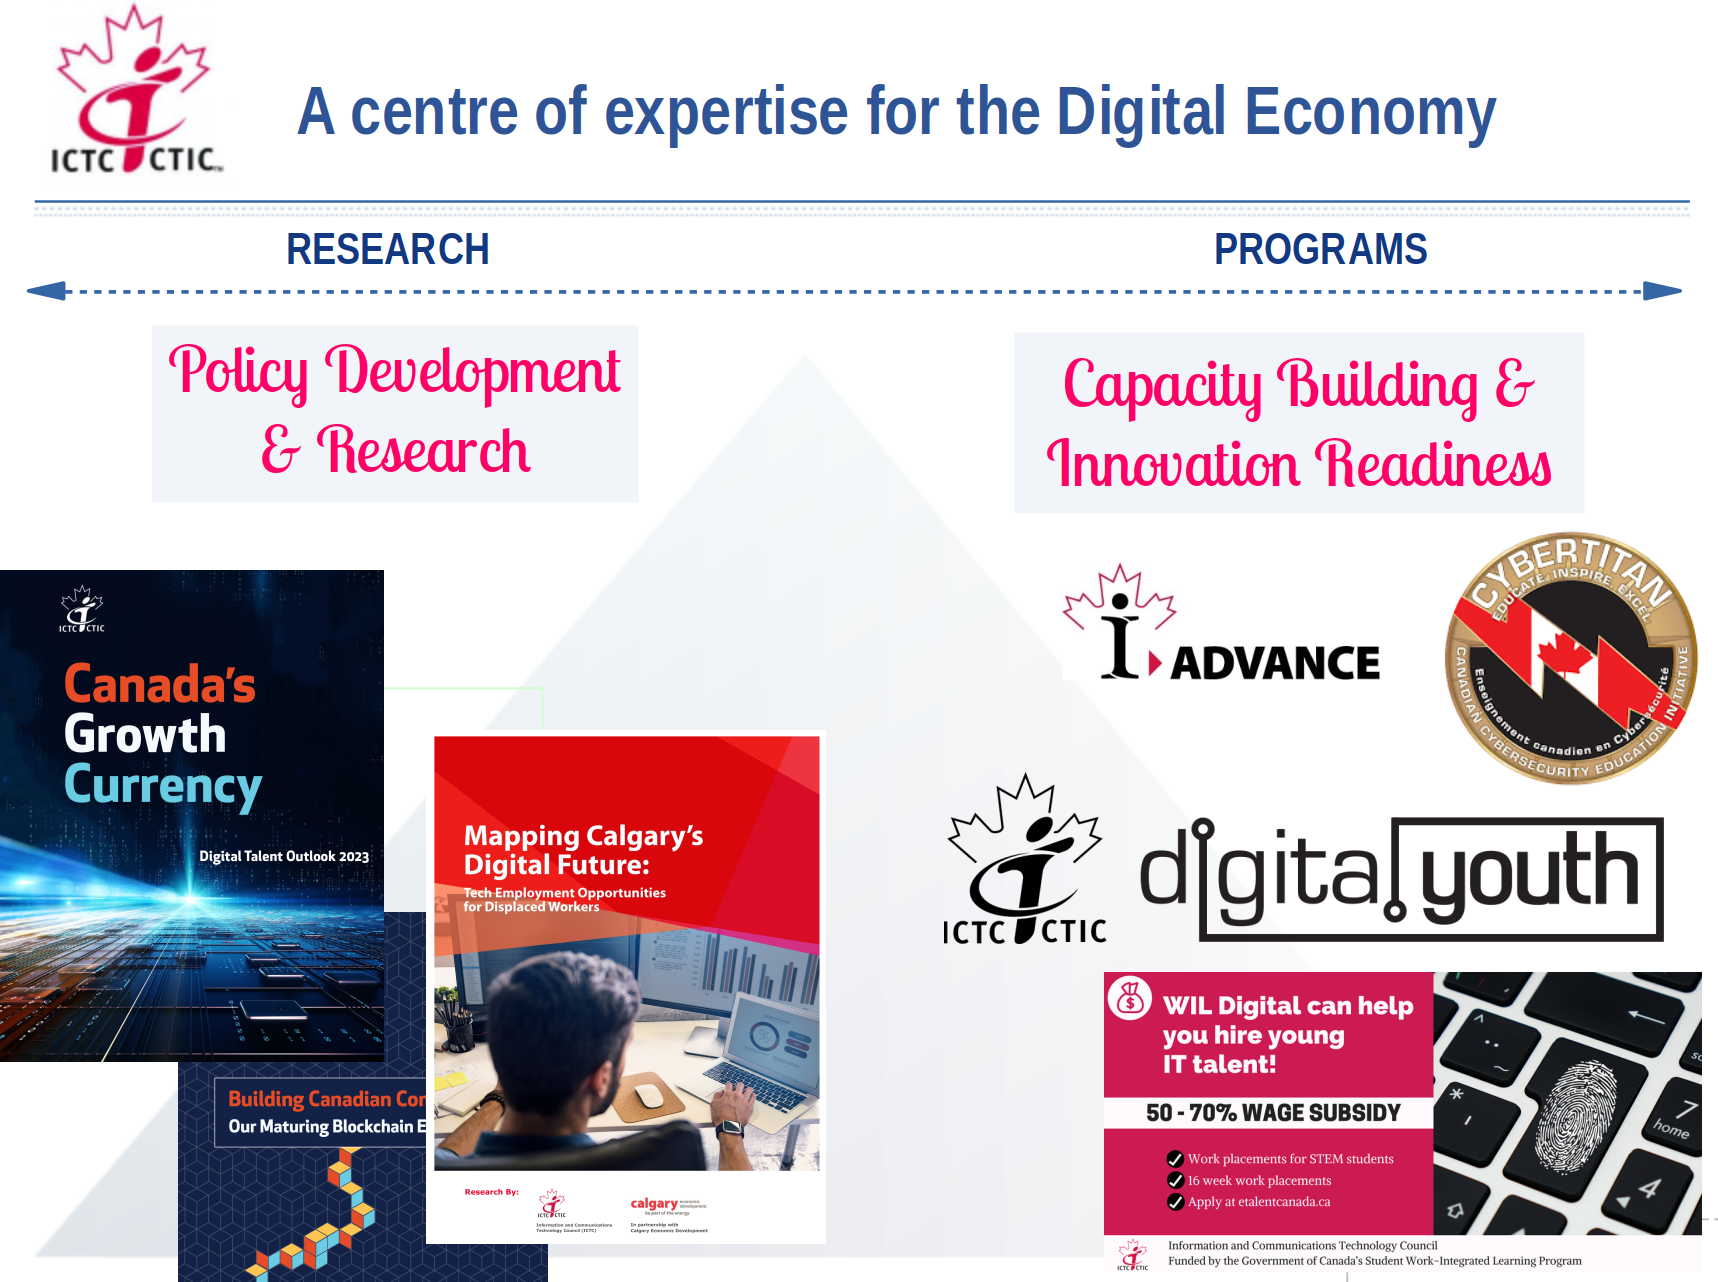
\includegraphics[width=11cm]{../../pics/ictc/ictc-at-a-glance}
	\caption{\tiny\url{https://www.ictc-ctic.ca}}
	\end{figure}
}

\frame{
  \frametitle{Leading the Blockchain supercluster bid (2017)}
	\begin{figure}
	
\includegraphics[width=11cm]{../../pics/ictc/blockchain2019/fabulousfive2}
	\end{figure}
	\begin{itemize}
    \item ICTC, ColliderX, Blockchain Research Institute, and the two Canadian Blockchain associations
    \item goals: education, startups, R\&D, international visibility and promotion
		\item raised \$50 million dollars in pledges
    \item raised visibility and interest with the Federal government (ISED)
	\end{itemize}
}

% ======================================================================================================
%                                    Blockchain industry in Canada 
% ======================================================================================================
\section{The Blockchain industry in Canada}

\frame{
  \frametitle{Report on the Blockchain industry in Canada}
  \begin{columns}[T]
  \column{0.5\textwidth}
%  \cite{ictc2019:blockchain}
	\begin{figure}
	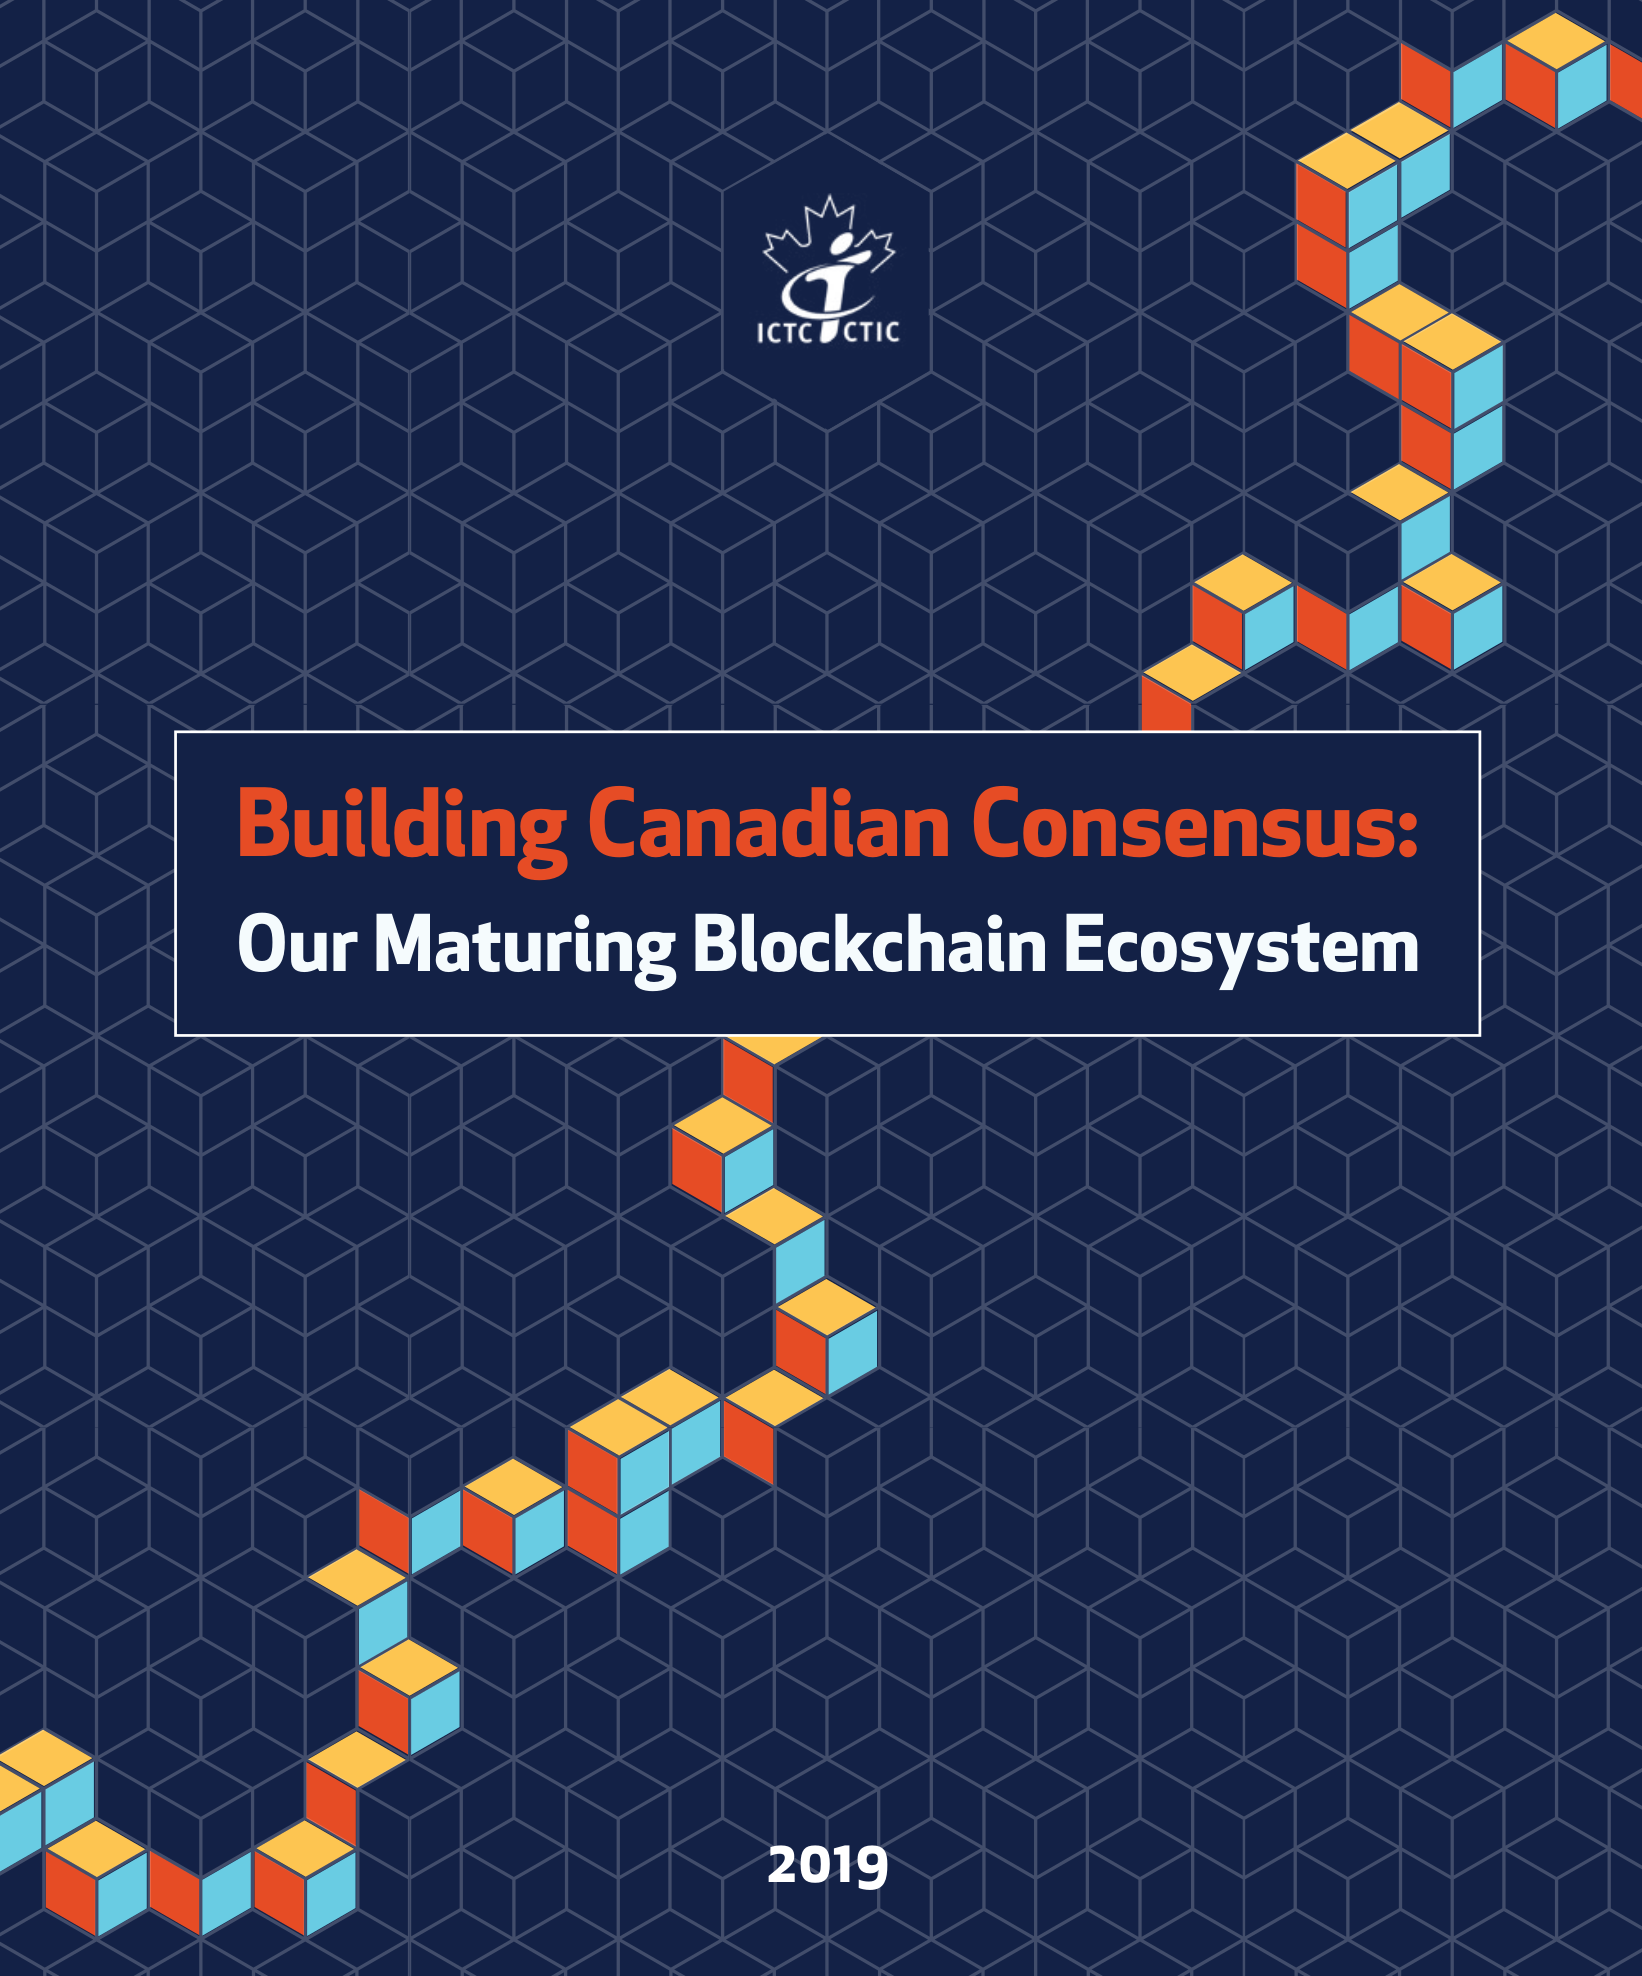
\includegraphics[height=6cm]{../../pics/ictc/blockchain2019/ictc-blockchain-cover}
	\end{figure}
  \column{0.5\textwidth}
    \vspace{2em}
    A national study on the state of the Blockchain industry and its ecosystem in Canada (\citeyear{ictc2019:blockchain}).\\
    \vspace{1em}
    We looked at 288 firms and 1,600 workers and their role.\\
    \vspace{1em}
    Source: Web (incl. job boards), plus 24 interviews, and two group discussions.
  \end{columns}
}

\frame{
	\frametitle{Blockchain in Canada}
	\begin{figure}
  \hspace*{-1.25cm}
	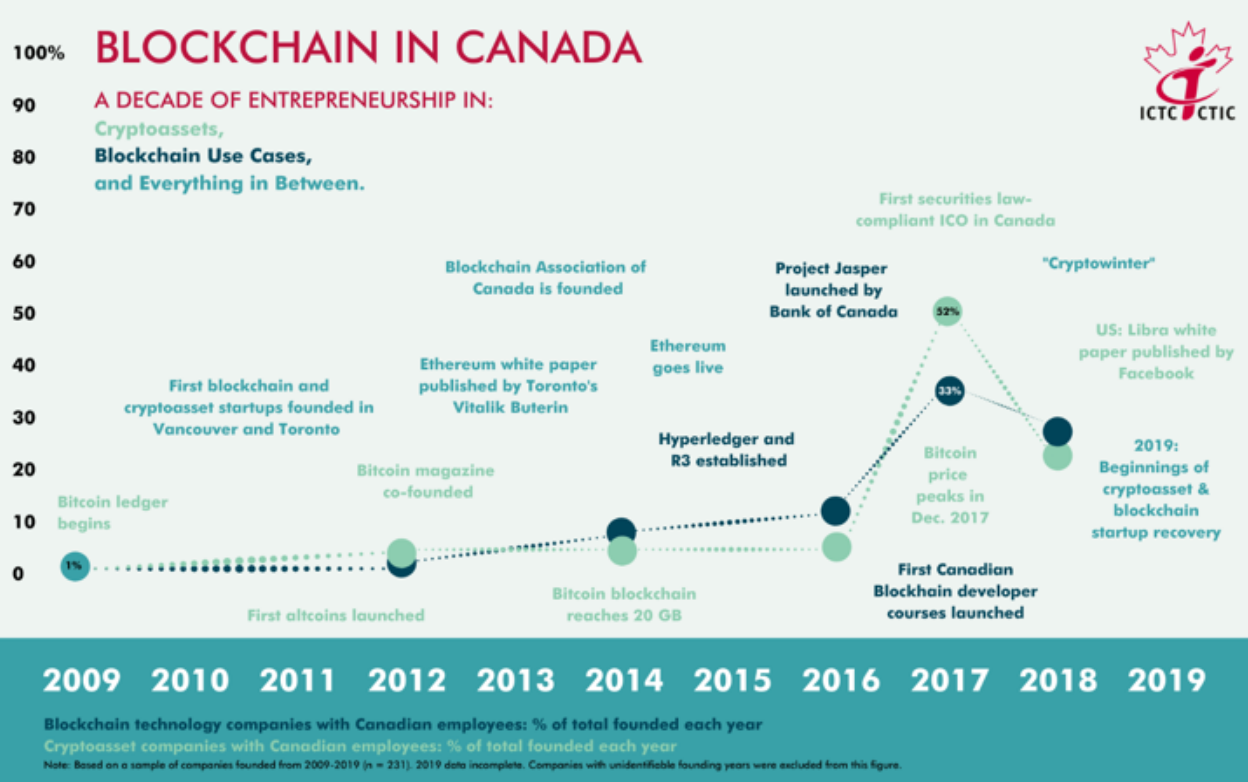
\includegraphics[width=11cm]{../../pics/ictc/blockchain2019/ictc-blockchain-in-canada-p19}
	%\caption{\tiny\url{https://www.ictc-ctic.ca}}
	\end{figure}
}

\frame{
	\frametitle{Industry applications}
	\begin{figure}
  \hspace*{-1.25cm}
	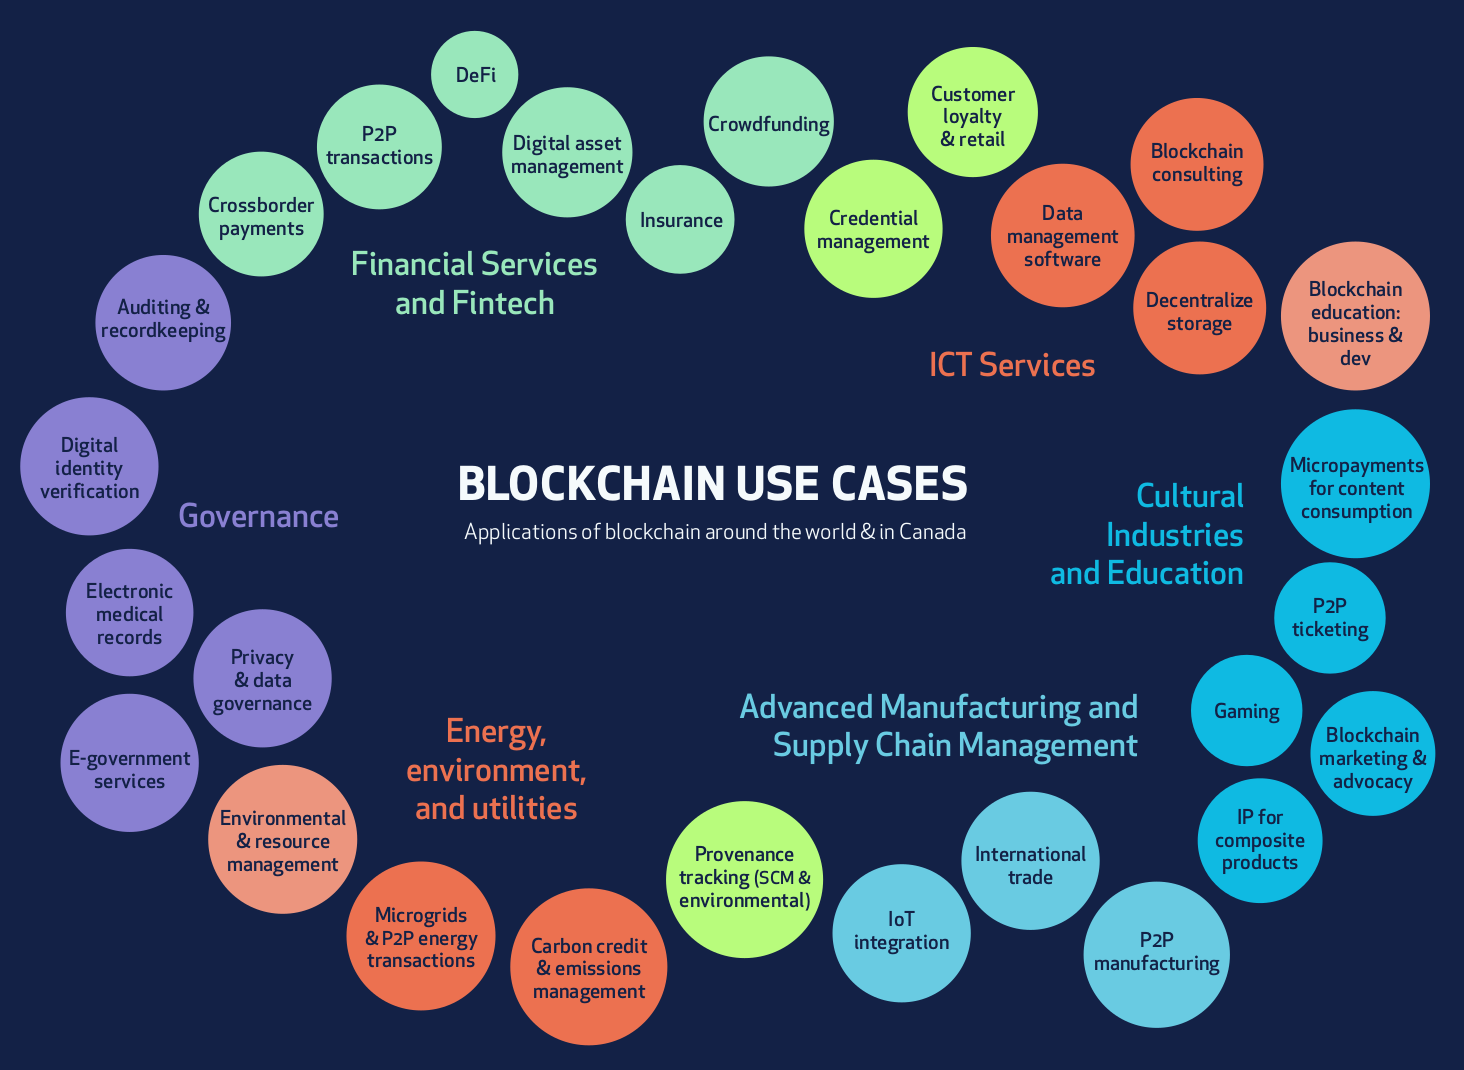
\includegraphics[width=11cm]{../../pics/ictc/blockchain2019/ictc-blockchain-usecases-p28}
	%\caption{\tiny\url{https://www.ictc-ctic.ca}}
	\end{figure}
}

\frame{
  \frametitle{Canadian companies per sector}
	\begin{figure}
  \hspace*{-1.25cm}
	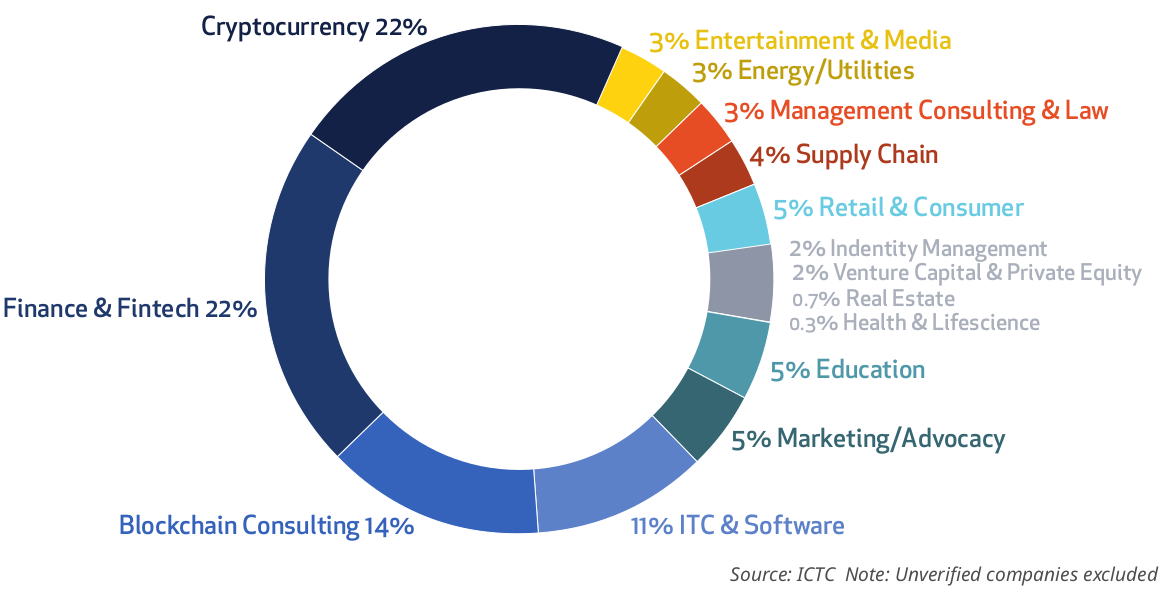
\includegraphics[width=11cm]{../../pics/ictc/blockchain2019/ictc-companies-per-sector-p24}
	%\caption{\tiny\url{https://www.ictc-ctic.ca}}
	\end{figure}
}

\frame{
  \frametitle{Canadian companies per sector}
	\begin{figure}
  \hspace*{-1.25cm}
	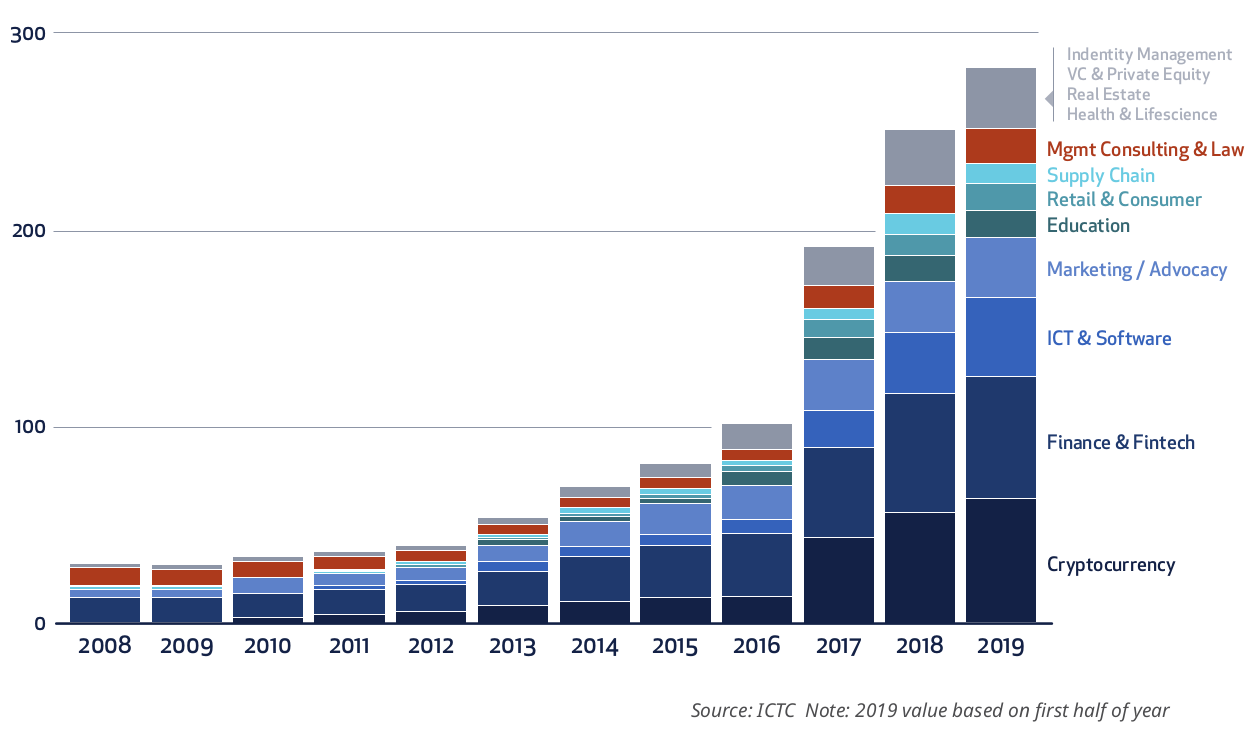
\includegraphics[width=11cm]{../../pics/ictc/blockchain2019/ictc-blockchain-sector-across-time-p25}
	%\caption{\tiny\url{https://www.ictc-ctic.ca}}
	\end{figure}
}

% ======================================================================================================
%                                     Regional differenciation
% ======================================================================================================
\section{Regional differentiation}
 

\frame{
  \frametitle{Regional expertise}
	\begin{figure}
  \hspace*{-1.25cm}
	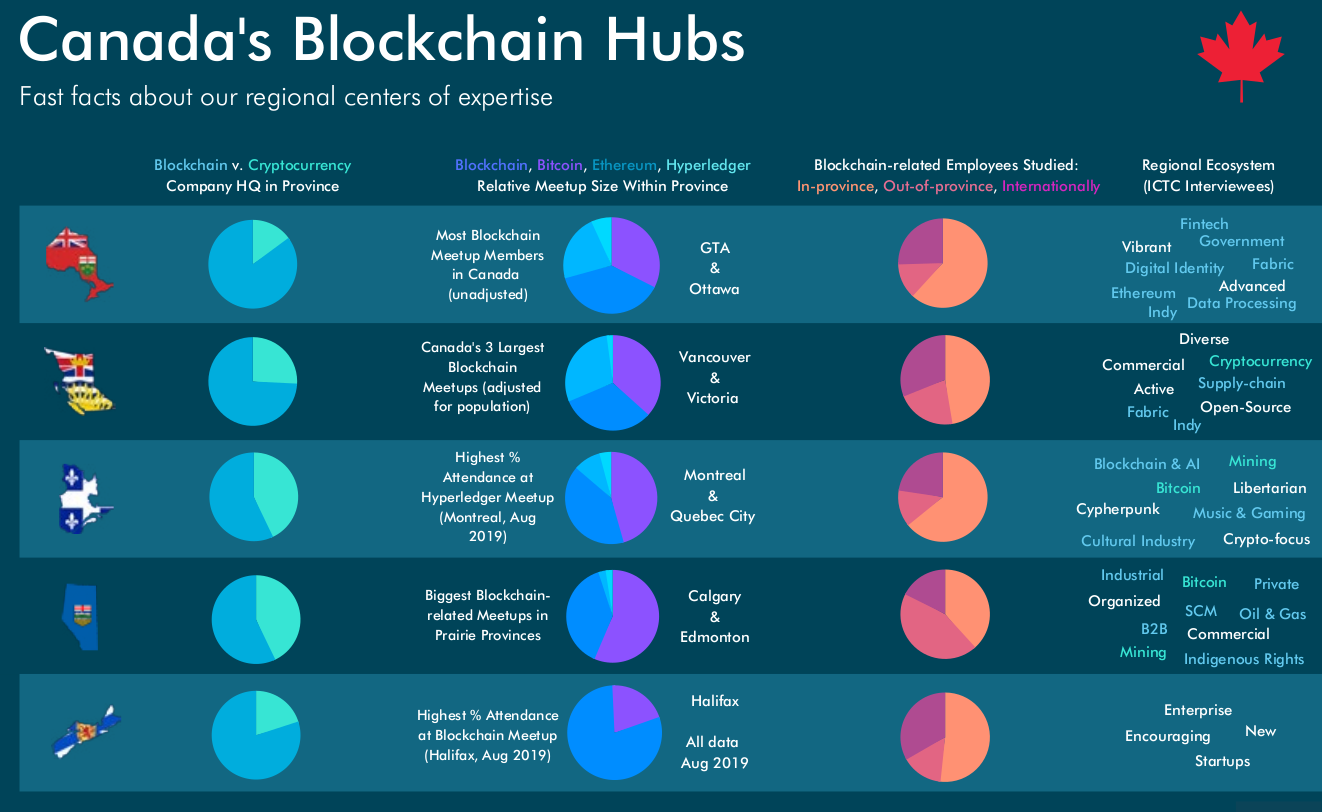
\includegraphics[width=11cm]{../../pics/ictc/blockchain2019/ictc-Canada-hubs-p31}
	%\caption{\tiny\url{https://www.ictc-ctic.ca}}
	\end{figure}
}

\frame{
  \frametitle{Regional expertise}
	\begin{figure}
  \hspace*{-1.25cm}
	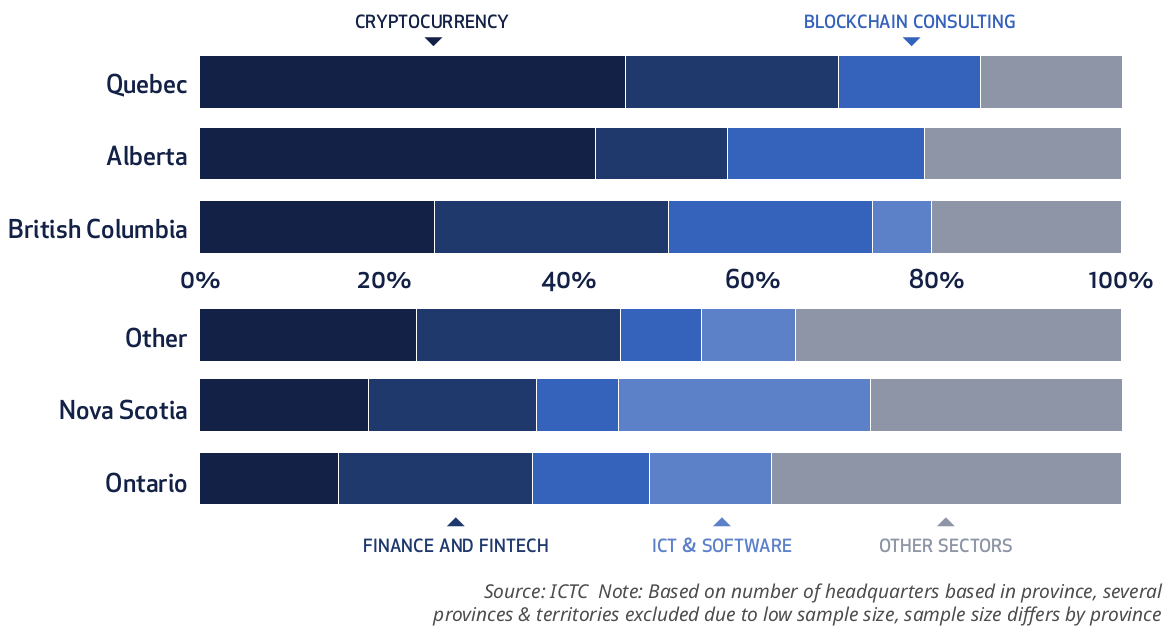
\includegraphics[width=11cm]{../../pics/ictc/blockchain2019/ictc-blockchain-cies-per-province-p34}
	%\caption{\tiny\url{https://www.ictc-ctic.ca}}
	\end{figure}
}

% ======================================================================================================
%                                     Labour \& Skills
% ======================================================================================================
\section{Labour market and Talent}

\frame{
  \frametitle{Worker occupation per sector}
	\begin{figure}
  \hspace*{-1.25cm}
	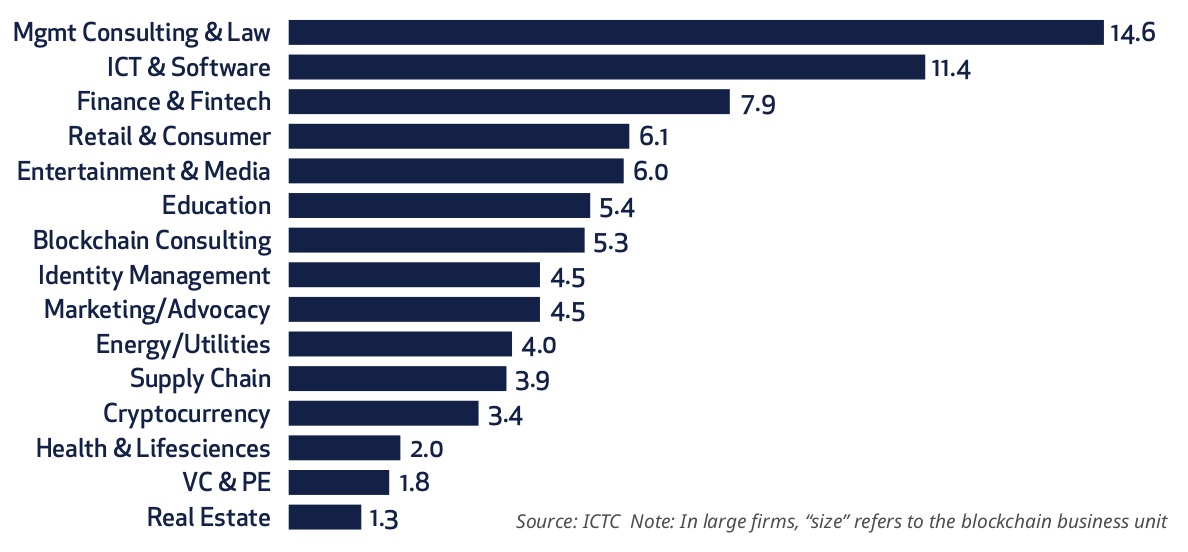
\includegraphics[width=11cm]{../../pics/ictc/blockchain2019/ictc-blockchain-workers-p30}
  \caption{\tiny\textit{Figure: Average number of Blockchain workers per company or Blockchain business unit, by Industry (Canada, 2019)}}
	\end{figure}
}

\frame{
  \frametitle{Top developer jobs in Blokchain}
	\begin{figure}
  \hspace*{-1.25cm}
	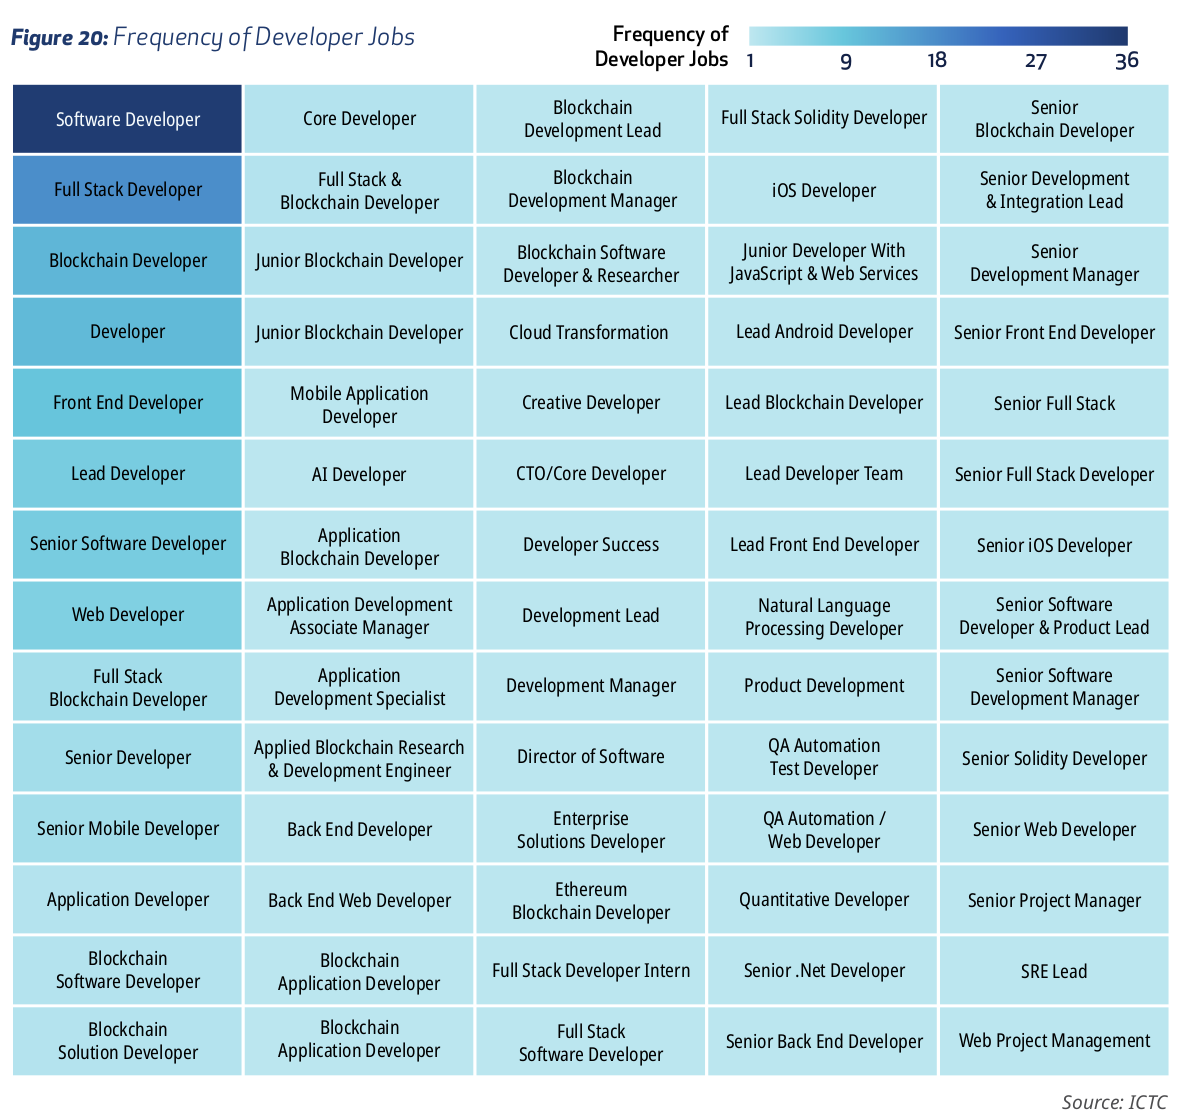
\includegraphics[height=8cm]{../../pics/ictc/blockchain2019/ictc-blockchain-devjobs-p44}
	%\caption{\tiny\url{https://www.ictc-ctic.ca}}
	\end{figure}
}

\frame{
  \frametitle{Follow the jobs}
	\begin{figure}
  \hspace*{-1.25cm}
	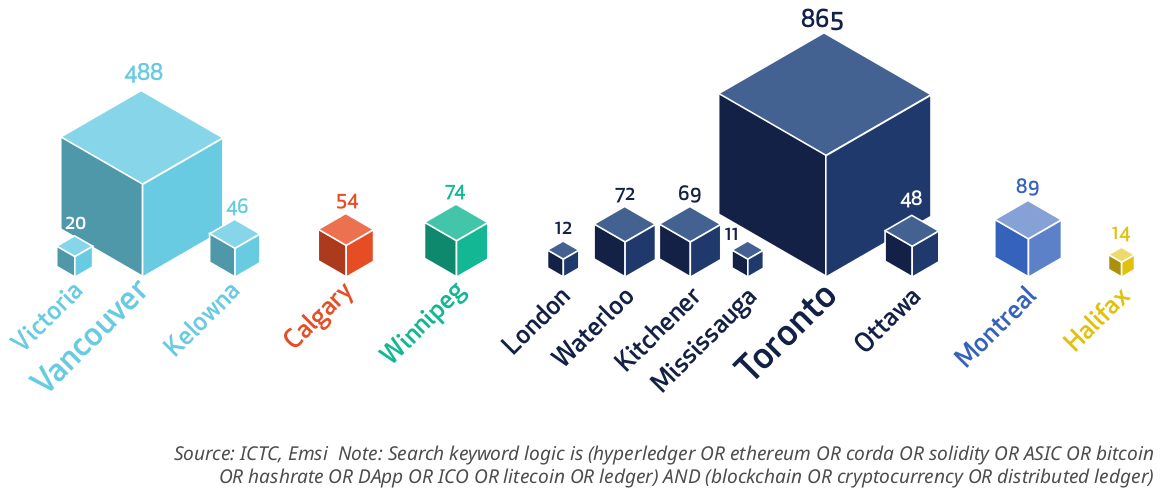
\includegraphics[width=11cm]{../../pics/ictc/blockchain2019/ictc-blockchain-job-posts-per-city-p35}
  \caption{\tiny\textit{Figure: The total number of jobs posted in each city from November 2017 to August 2019}}
	\end{figure}
}

\frame{
  \frametitle{Skills in high demand}
	\begin{figure}
  \hspace*{-1.25cm}
	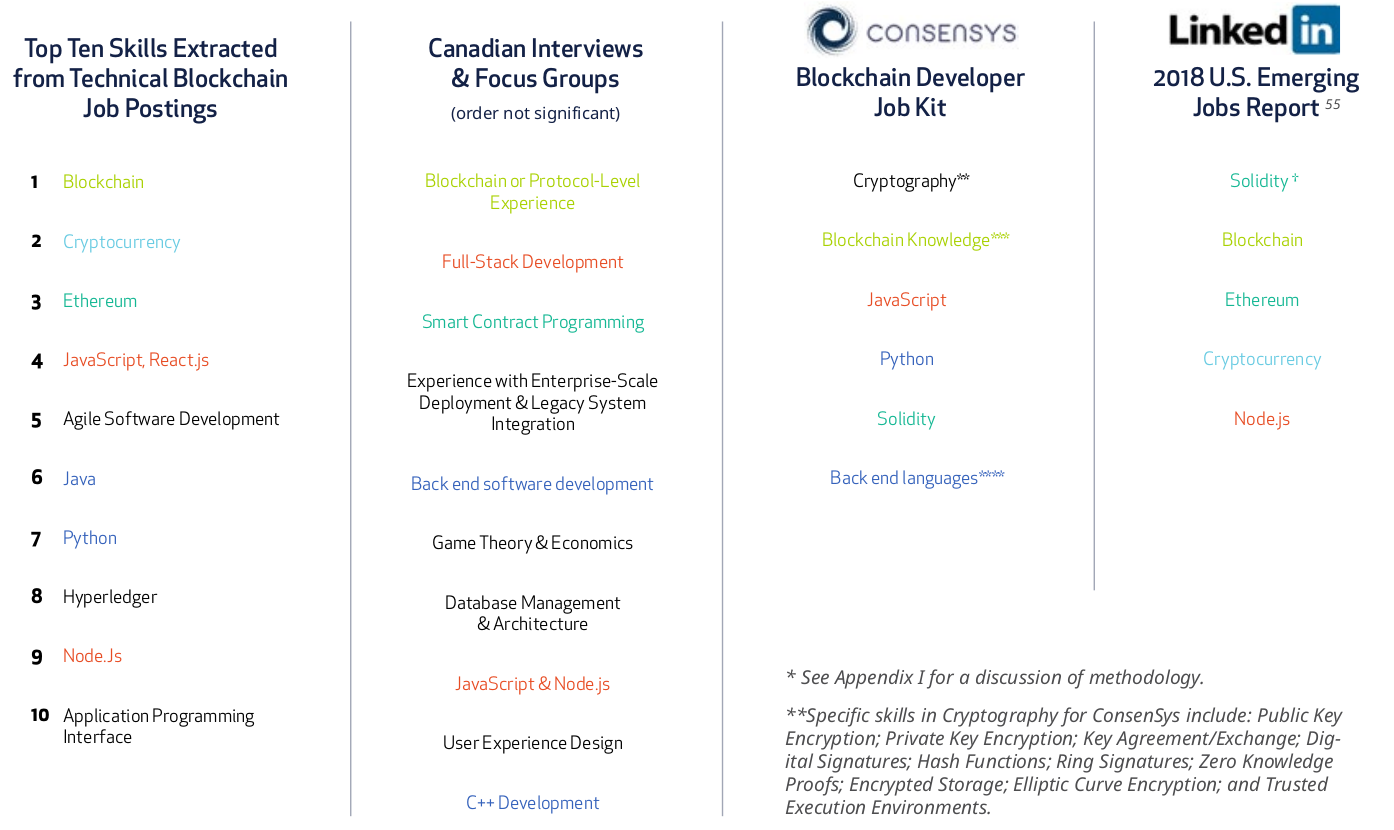
\includegraphics[width=11cm]{../../pics/ictc/blockchain2019/ictc-blockchain-competencies-p48}
	%\caption{\tiny\url{https://www.ictc-ctic.ca}}
	\end{figure}
}

\frame{
  \frametitle{Education}
	\begin{figure}
  \hspace*{-1.25cm}
	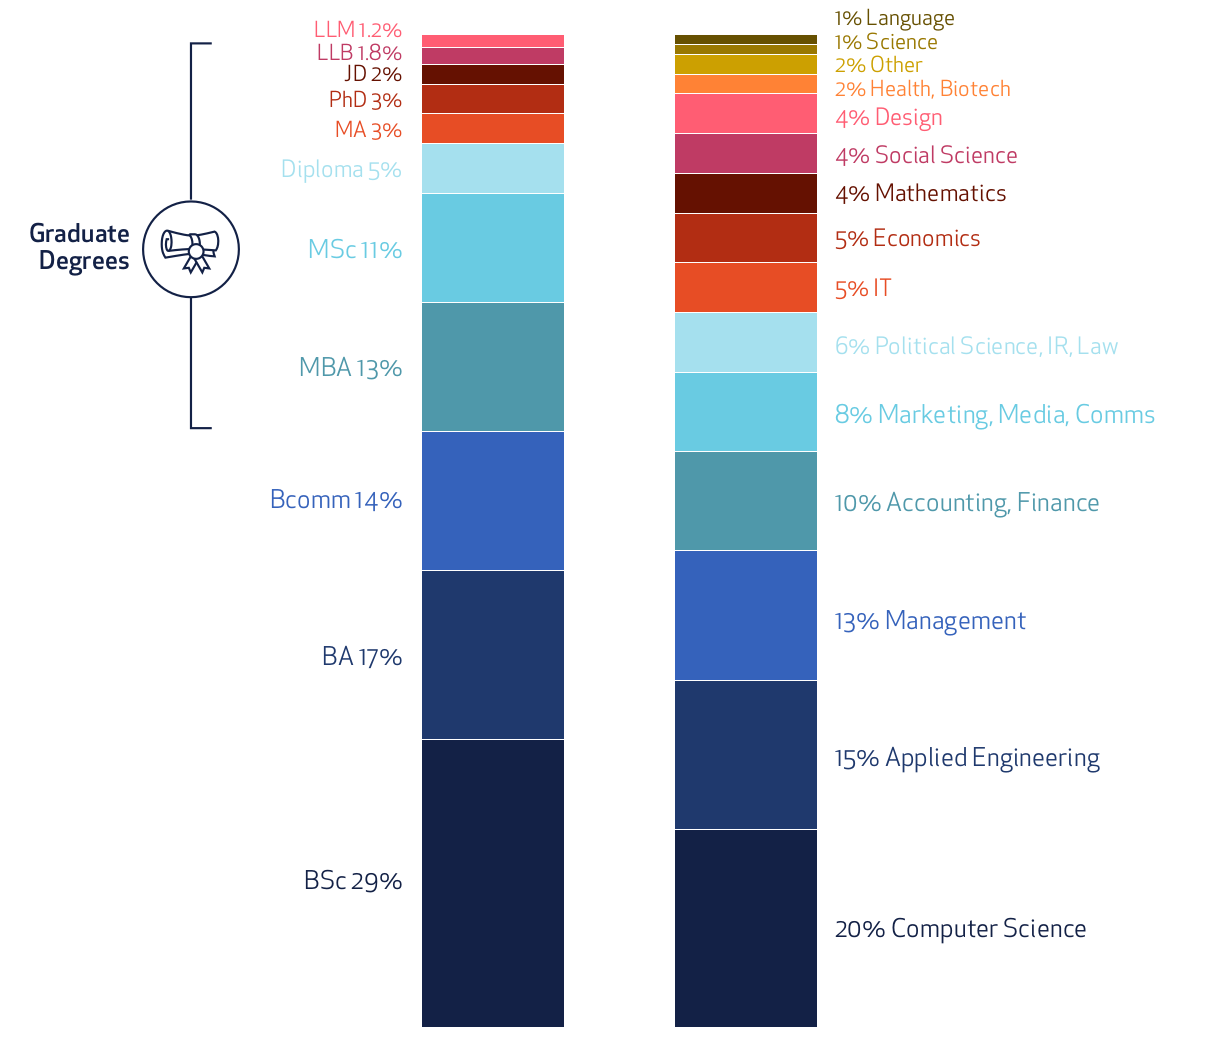
\includegraphics[height=8cm]{../../pics/ictc/blockchain2019/ictc-blockchain-education-p40}
	%\caption{\tiny\url{https://www.ictc-ctic.ca}}
	\end{figure}
}

\frame{
  \frametitle{Aiming for parity}
	\begin{figure}
  \hspace*{-1.25cm}
	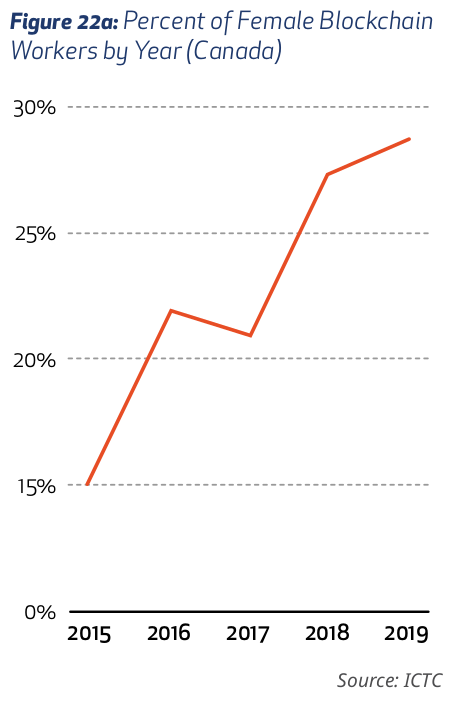
\includegraphics[height=7cm]{../../pics/ictc/blockchain2019/ictc-blockchain-female-p45}
	%\caption{\tiny\url{https://www.ictc-ctic.ca}}
	\end{figure}
}

% ======================================================================================================
%                                     Startups and New Ventures
% ======================================================================================================
\section{Startups and new ventures}

%\frame{
%  \frametitle{Types of firms}
%	\begin{figure}
%  \hspace*{-1.25cm}
%	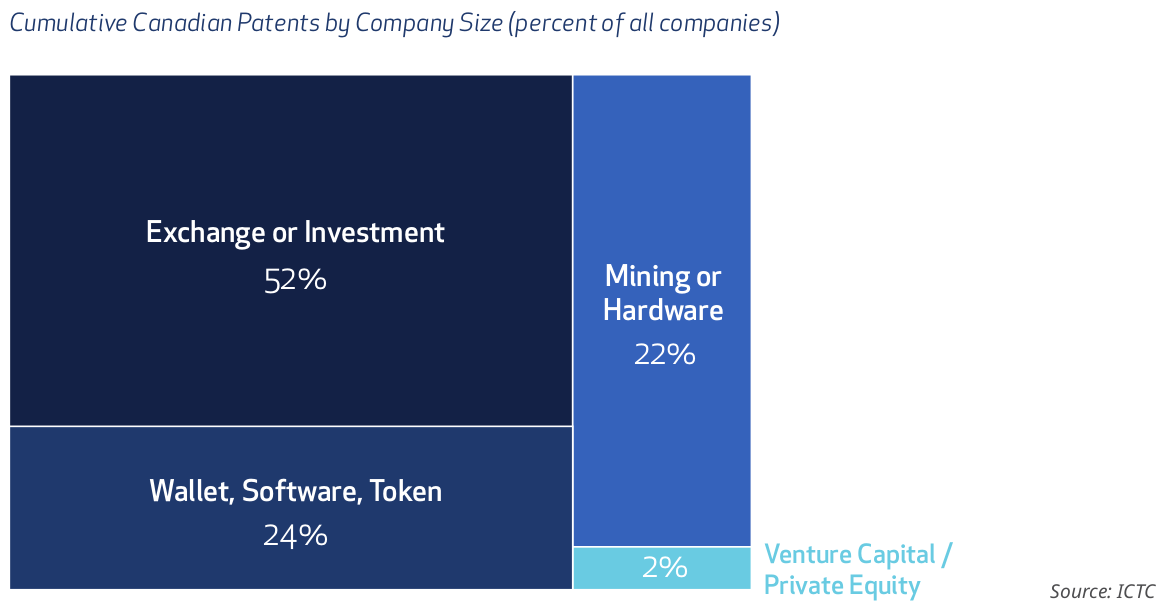
\includegraphics[width=11cm]{../../pics/ictc/blockchain2019/ictc-blockchain-canadian-patents-cie-size-p62}
%	\caption{\tiny Proportions of types of cryptocurrency-related firms in our dataset}
%	\end{figure}
%}

\frame{
  \frametitle{Creation of Intellectual Property}
	\begin{figure}
  \hspace*{-1.25cm}
	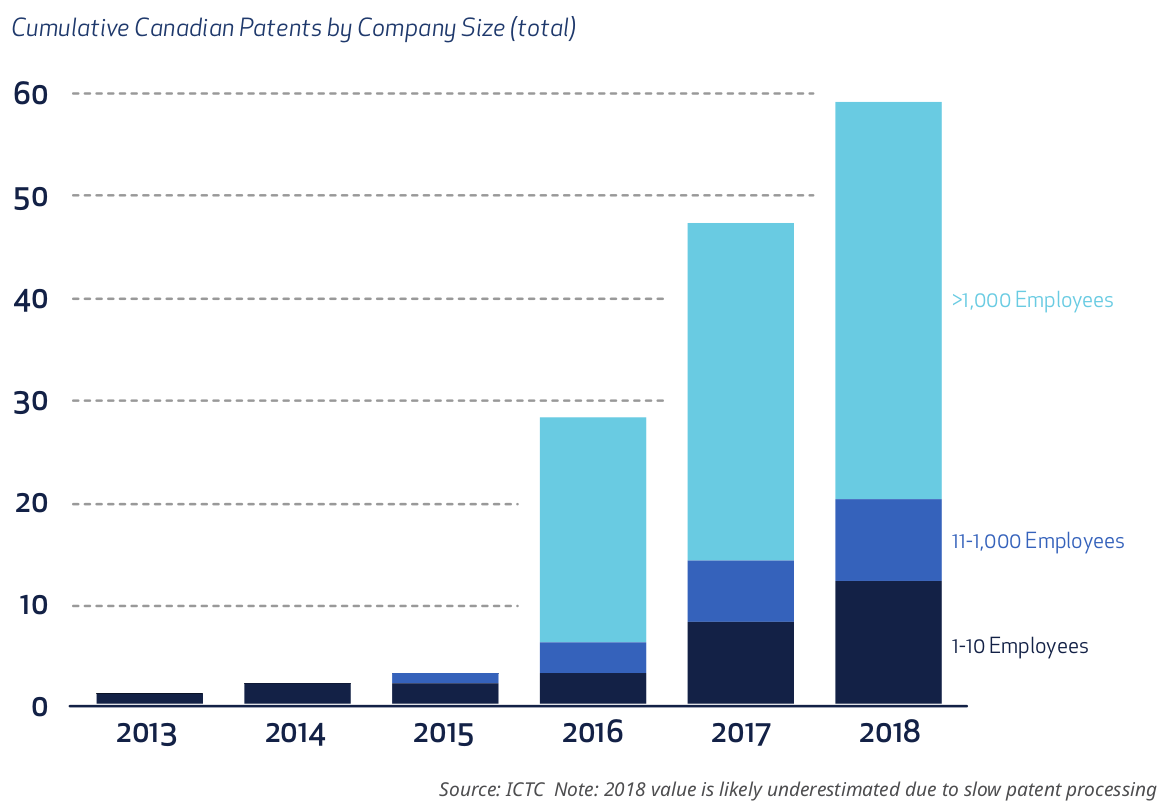
\includegraphics[width=11cm]{../../pics/ictc/blockchain2019/ictc-blockchain-canadian-patents-cumulative-p62}
	%\caption{\tiny\url{https://www.ictc-ctic.ca}}
	\end{figure}
}

\frame{
  \frametitle{Smaller firms are gaining ground on creating Intellectual Property}
	\begin{figure}
  \hspace*{-1.25cm}
	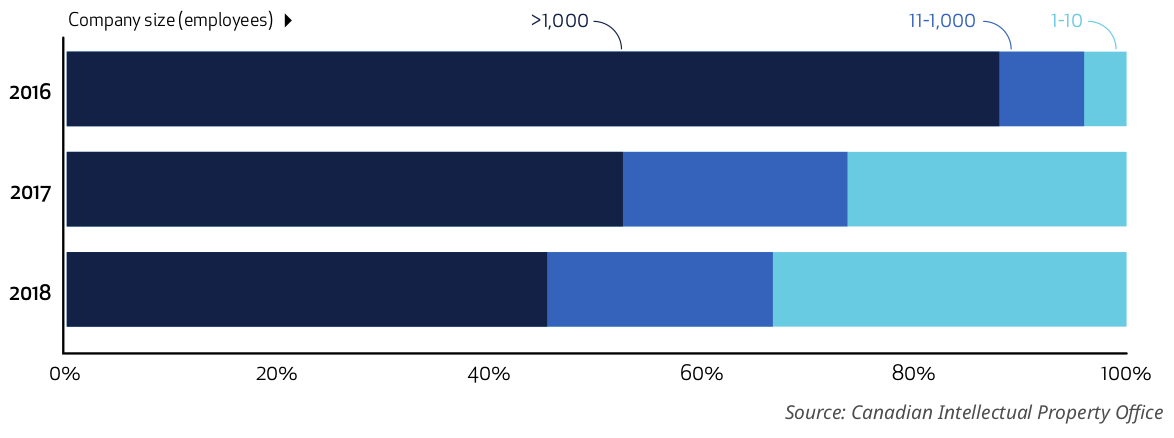
\includegraphics[width=11cm]{../../pics/ictc/blockchain2019/ictc-blockchain-canadian-patents-p55}
	%\caption{\tiny\url{https://www.ictc-ctic.ca}}
	\end{figure}
}

\frame{
  \frametitle{Startups are maturing}
	\begin{figure}
  \hspace*{-1.25cm}
	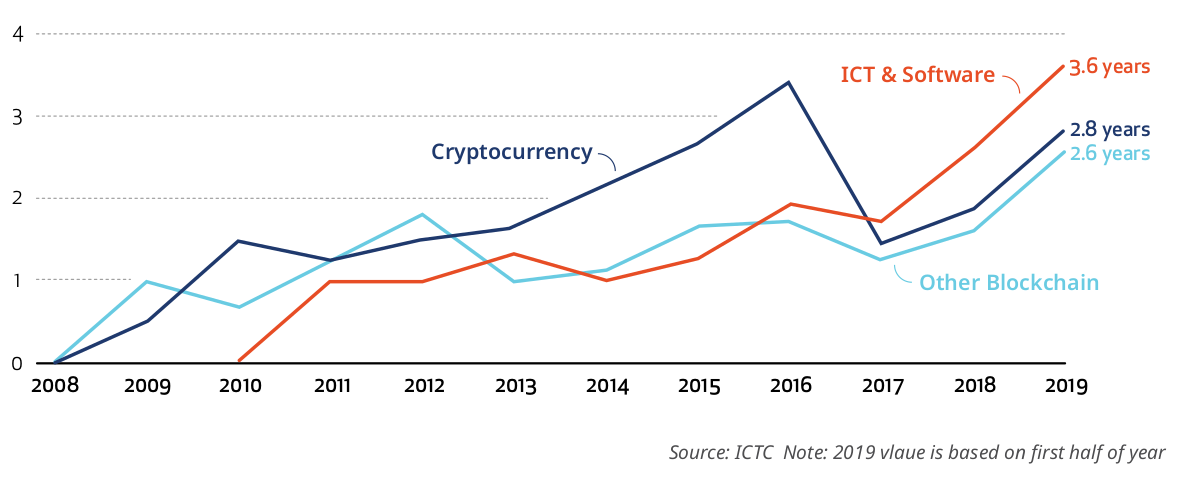
\includegraphics[width=11cm]{../../pics/ictc/blockchain2019/ictc-blockchain-firms-age-p57}
  \caption{\tiny\textit{Figure: Average age of Blockchain firms funded after 2008 (Canada)}}
	\end{figure}
}

\frame{
  \frametitle{Startups are maturing}
	\begin{figure}
  \hspace*{-1.25cm}
	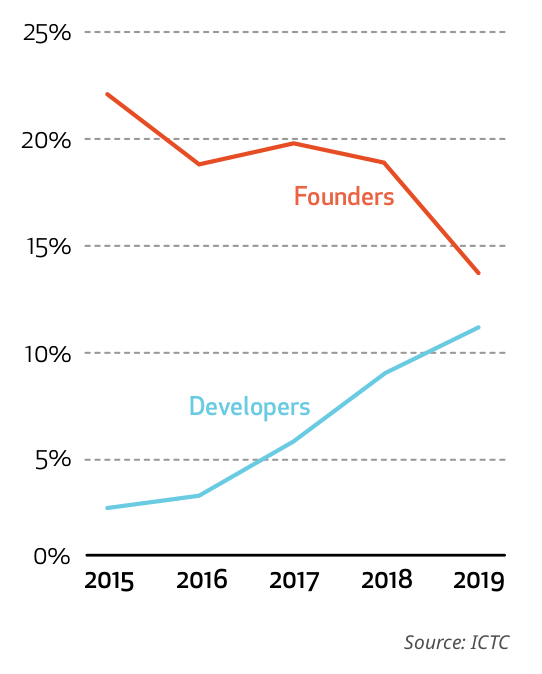
\includegraphics[height=7cm]{../../pics/ictc/blockchain2019/ictc-blockchain-roles-p43}
	\end{figure}
}

\frame{
  \frametitle{Startups are maturing}
	\begin{figure}
  \hspace*{-1.25cm}
	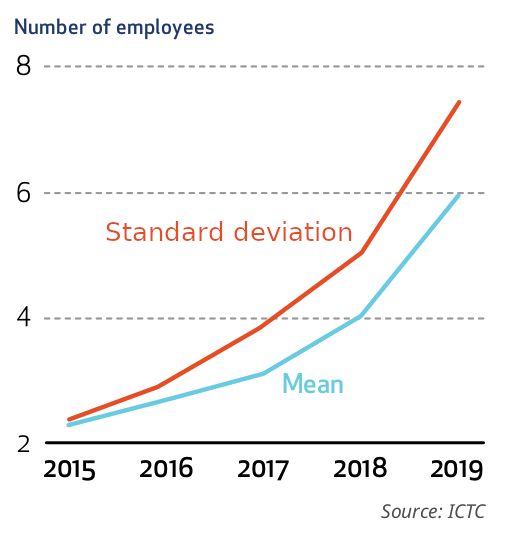
\includegraphics[height=7cm]{../../pics/ictc/blockchain2019/ictc-blockchain-cie-size-p44}
	%\caption{\tiny\url{https://www.ictc-ctic.ca}}
	\end{figure}
}

% ======================================================================================================
%                                     Adoption and Change Management
% ======================================================================================================
\section{Adoption in organizations}


\frame{
  \frametitle{Convergence}
  \framesubtitle{of disruptive technologies and practices leads to exponential growth}
  \begin{columns}[T]
  \column{0.5\textwidth}
%  \cite{ictc2019:blockchain}
	\begin{figure}
  %\captionsetup{justification=centering,margin=2cm}
  \captionsetup{justification=centering}
	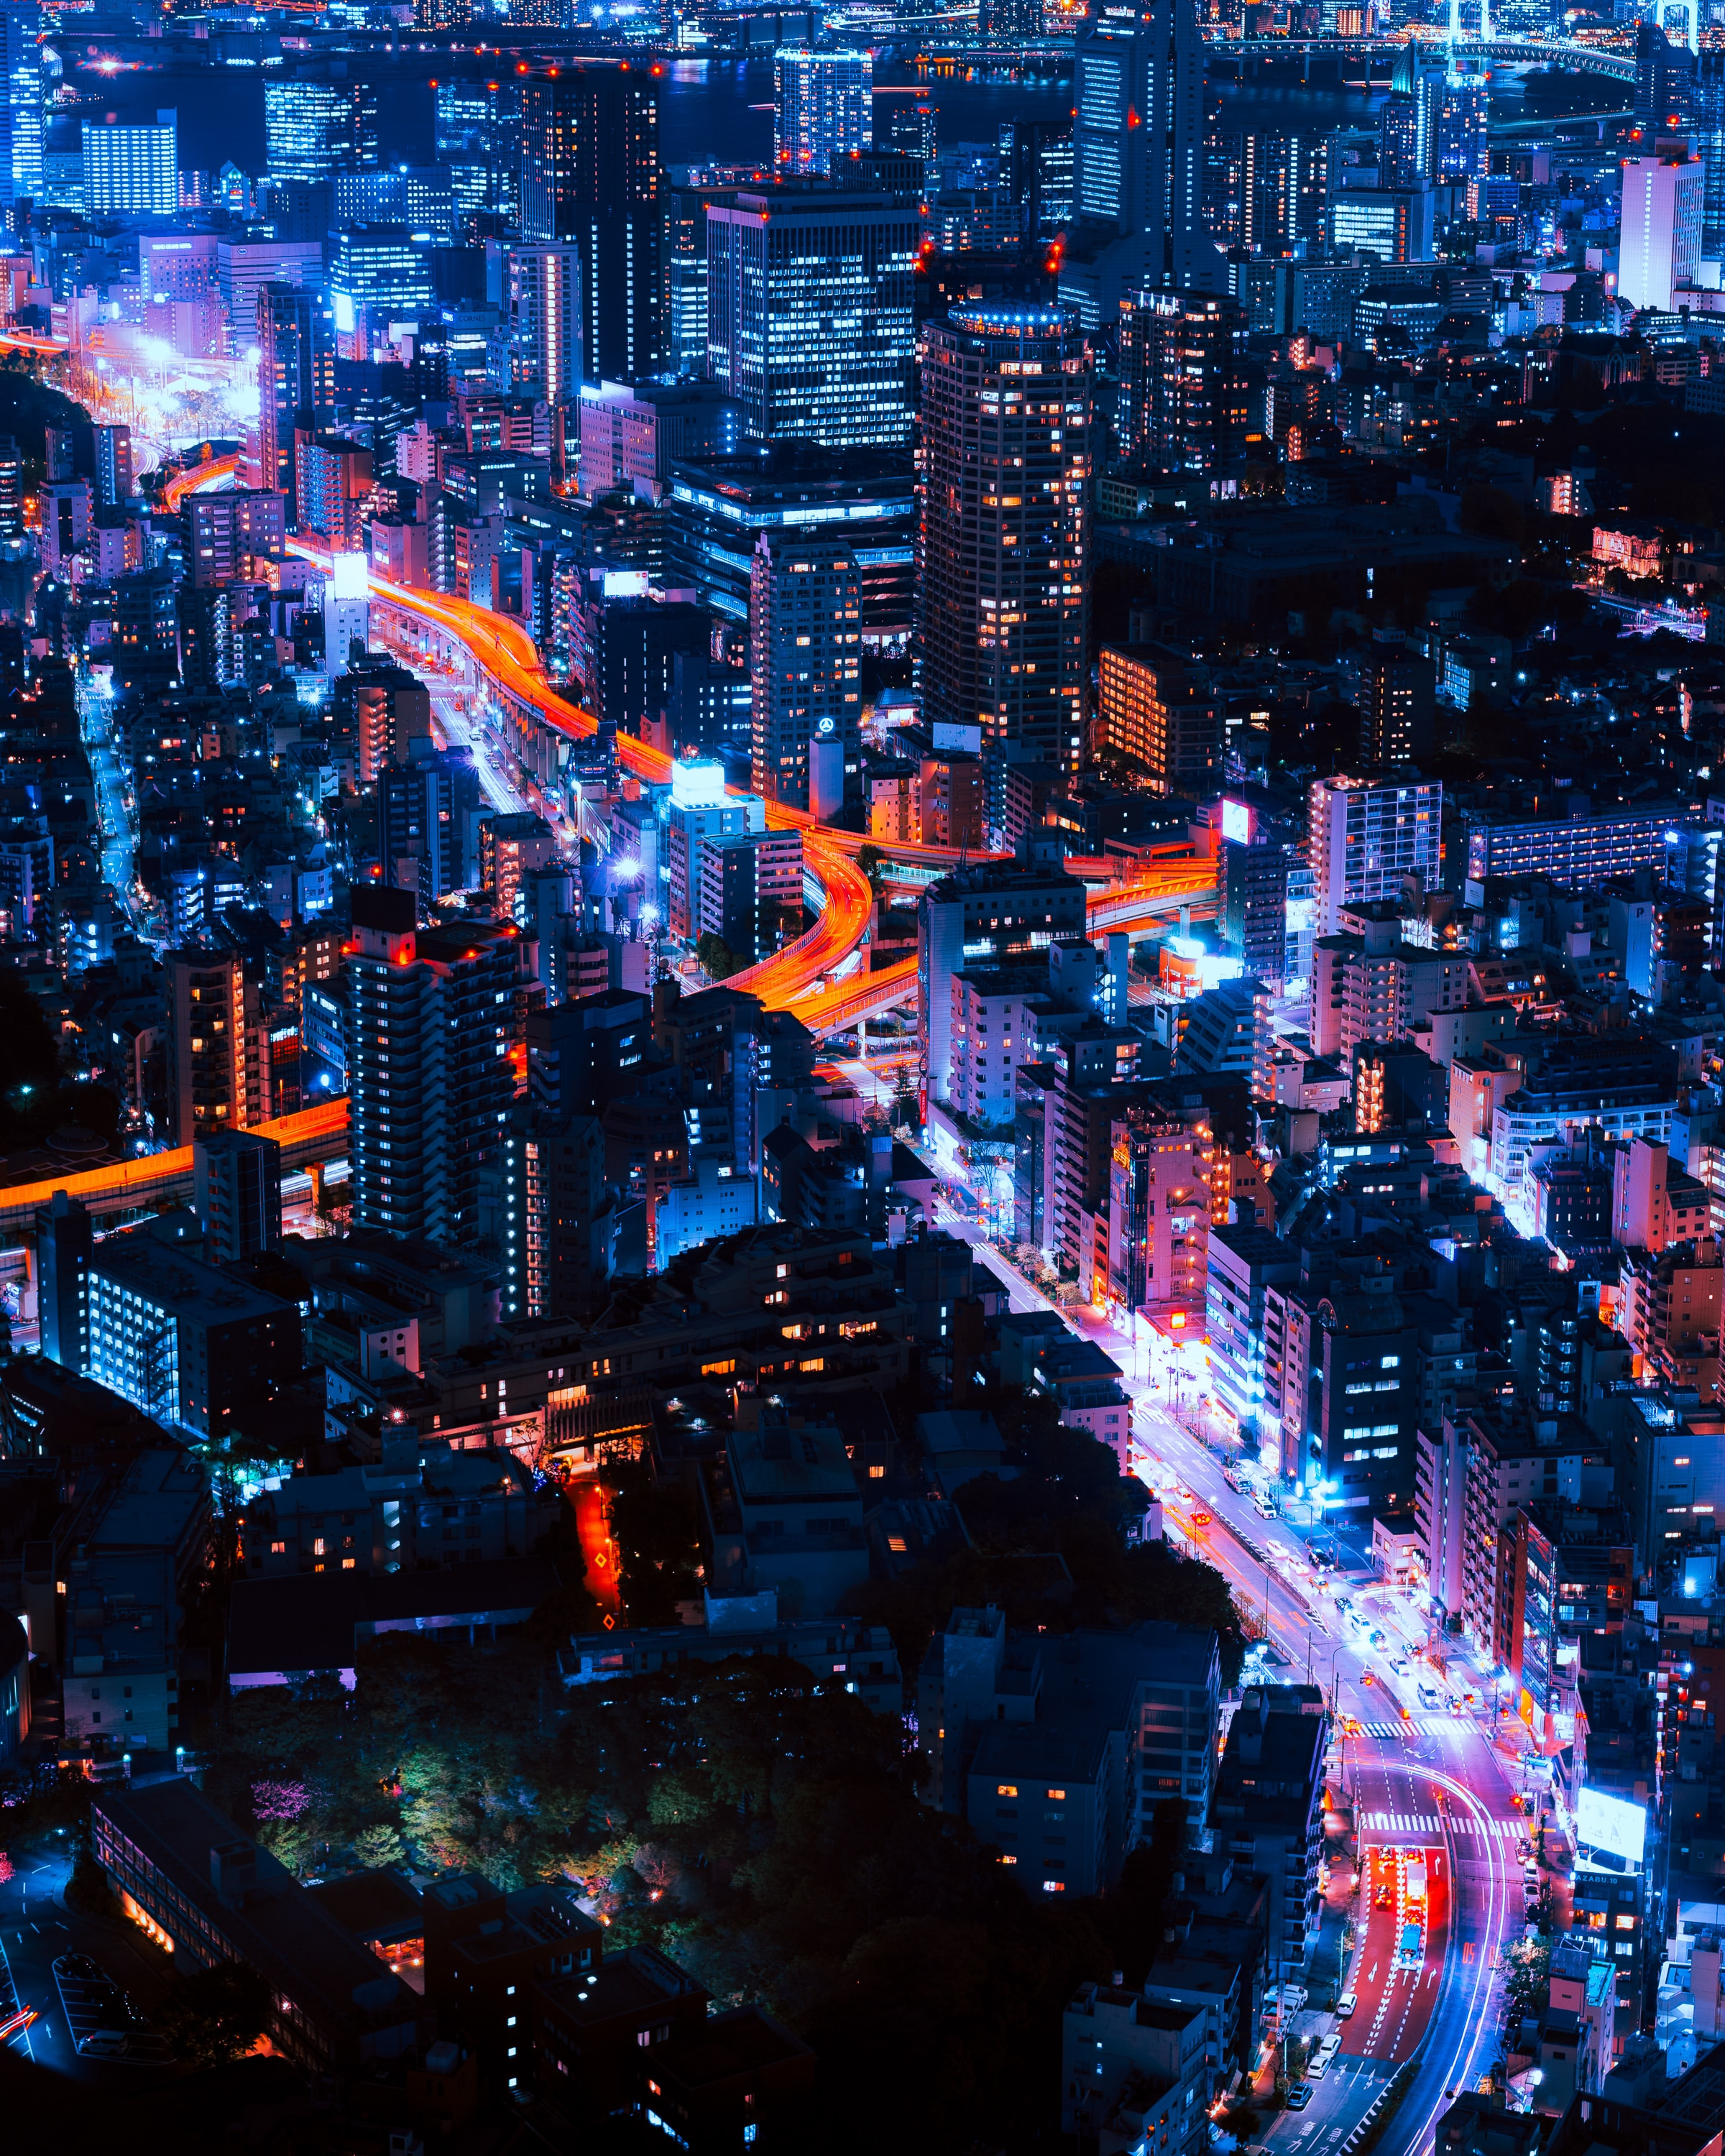
\includegraphics[height=6cm]{../../pics/convergence/pawel-nolbert-4u2U8EO9OzY-unsplash}
  \caption{\tiny\textit{Photo: credit goes to Pawel Nolbert (Unsplash)}}
	\end{figure}
  \column{0.5\textwidth}
    \vspace{2em}
    \begin{itemize}
      \item Blockchain
      \item AI
      \item 5G
      \item IoT
      \item Open collaboration
    \end{itemize}
  \end{columns}
}

\frame{
  \frametitle{Focus on business value}
  \begin{columns}[T]
  \column{0.5\textwidth}
	\begin{figure}
  %\captionsetup{justification=centering,margin=2cm}
  \captionsetup{justification=centering}
	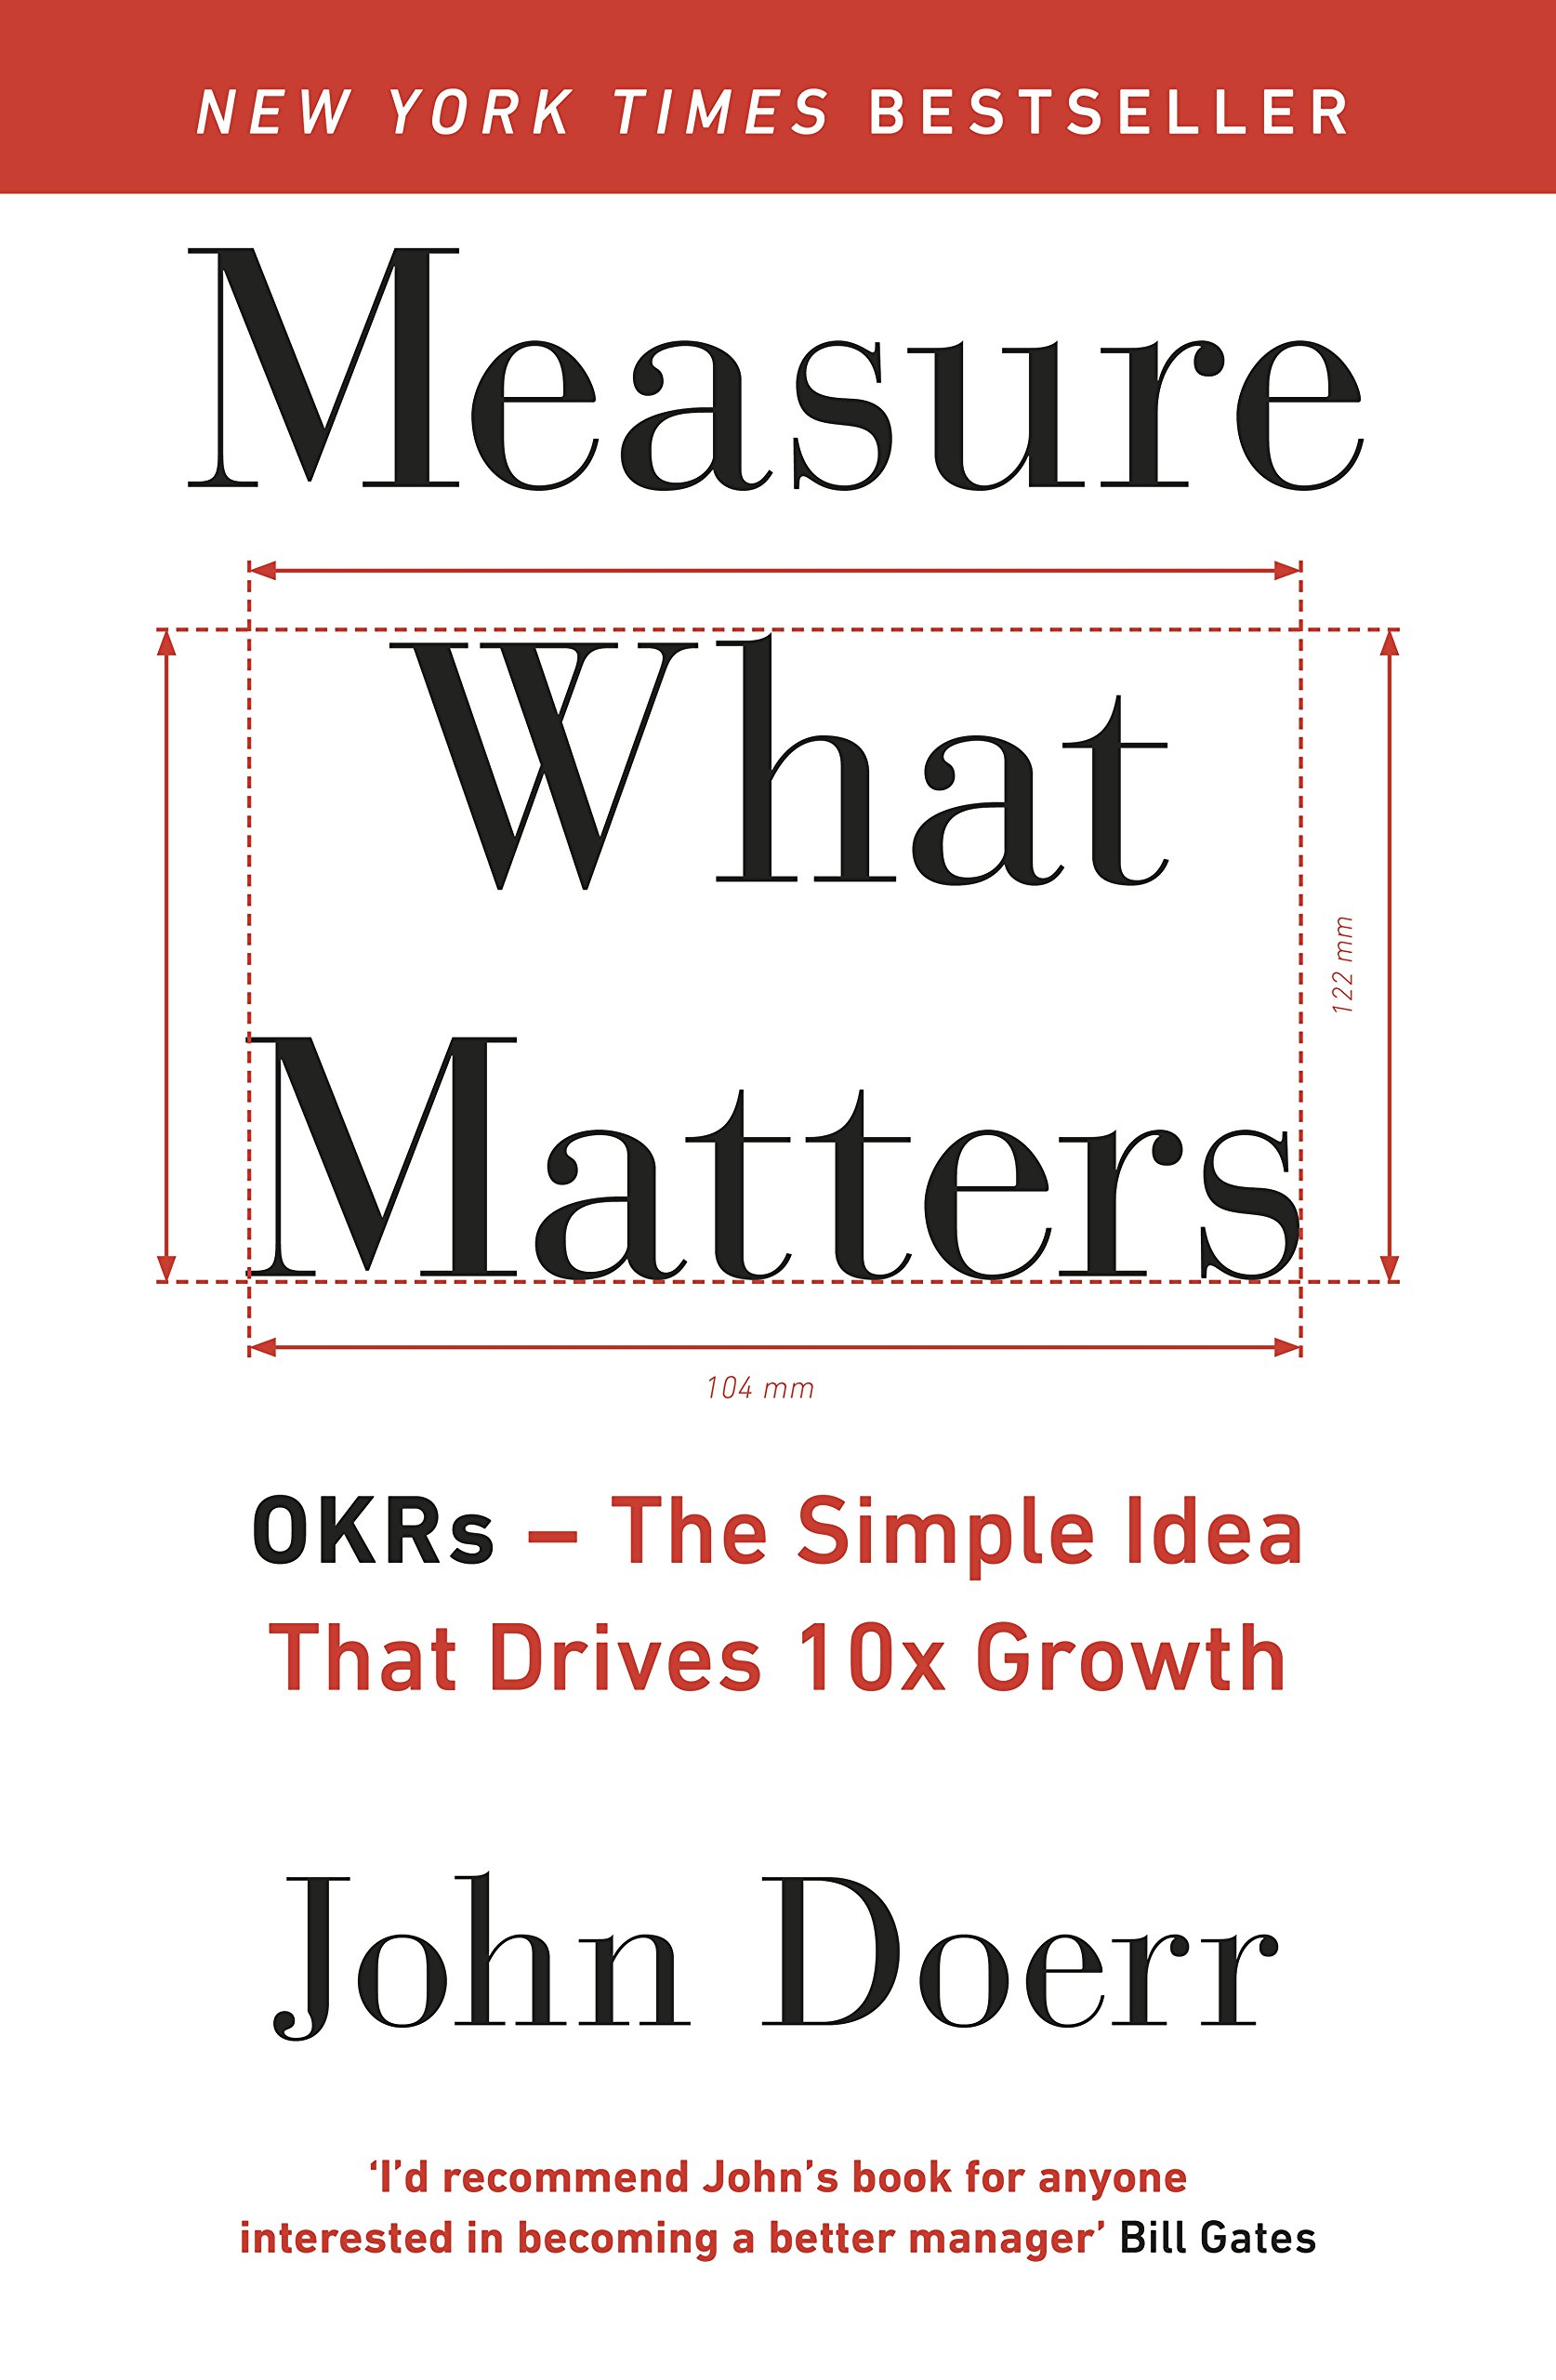
\includegraphics[height=6cm]{../../pics/transformation/okr-book}
  \caption{\tiny Ted Talk intro at \url{https://www.youtube.com/watch?v=L4N1q4RNi9I}}
	\end{figure}
  \column{0.5\textwidth}
    \vspace{2em}
    Fiercely pursuing objectives that matter, breaking down silos, taking calculated risks are necessary conditions for an effective transformation.\\
    \vspace{1em}
    \pause
    Internal convergence ("Collective Genius", \citeauthor{hbr2014:collectivegenius}, \citeyear{hbr2014:collectivegenius}):
    \begin{itemize}
      \item domain expertise
      \pause
      \item freedom to innovate
      \pause
      \item freedom to fail (fast) 
      \pause
       \item big bets
    \end{itemize}
  \end{columns}
}

\frame{
  \frametitle{WIL Digital}
  \framesubtitle{Accelerating innovation in key sector to boost the digital economy in Canada}
  \begin{columns}[T]
  \column{0.5\textwidth}
	\begin{figure}
  %\captionsetup{justification=centering,margin=2cm}
  %\captionsetup{justification=centering}
	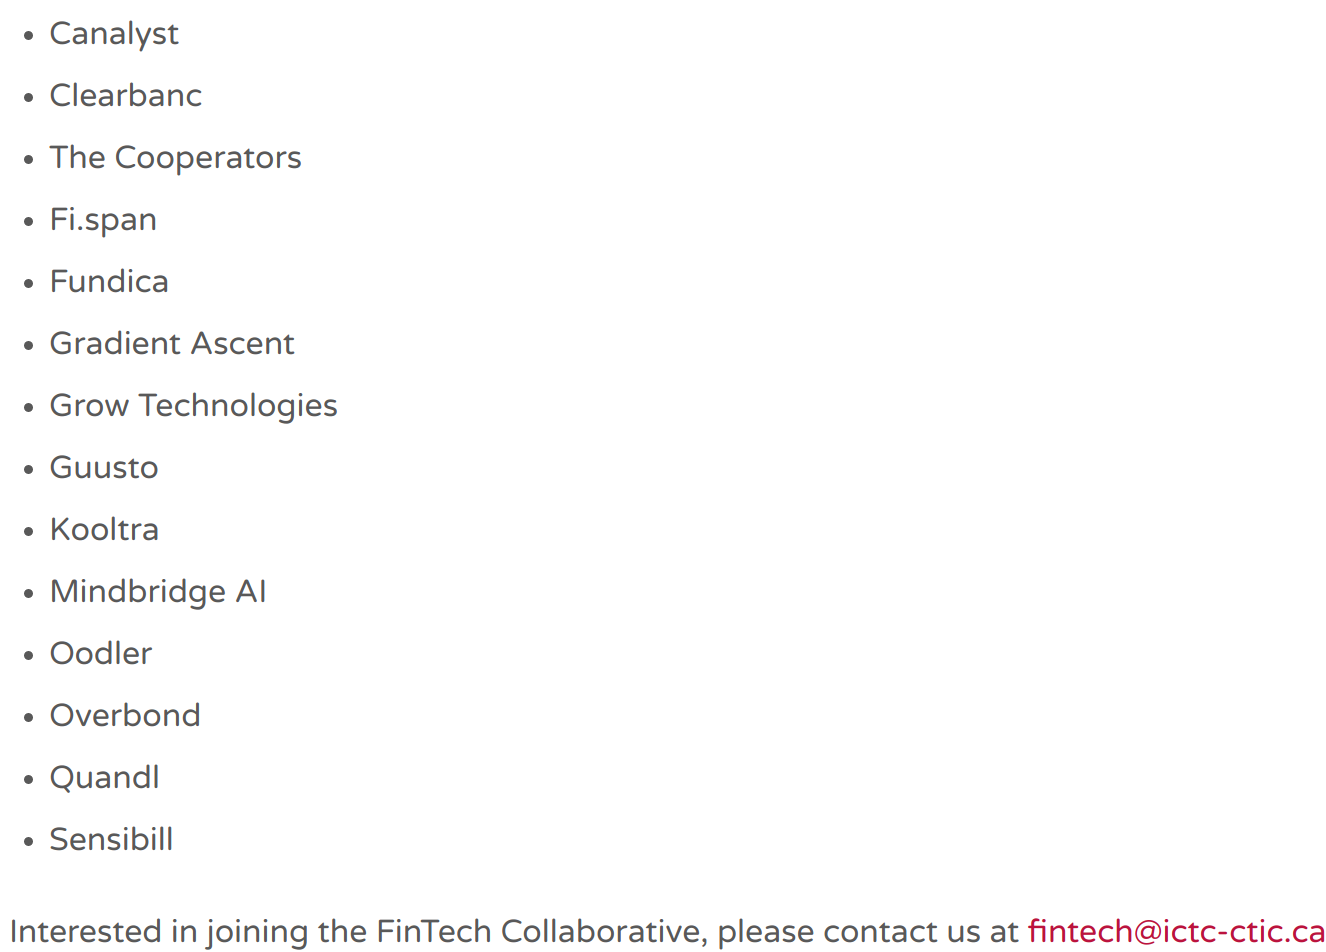
\includegraphics[height=6cm]{../../pics/ictc/wil/fintech-collaborative}
  \caption{\tiny\url{https://www.ictc-ctic.ca/upskilling-canadian-post-secondary-students-strengthening-fintech-industry/}}
	\end{figure}
  \column{0.5\textwidth}
    \vspace{2em}
    ICTC's WIL Digital program focuses on key sectors highlighted by our research:
    \begin{itemize}
      \item \href{https://www.ictc-ctic.ca/upskilling-canadian-post-secondary-students-strengthening-fintech-industry/}{FinTech} (see on the left)
      \item IoT
      \item \href{https://www.stageencommerce.ca}{Intelligent Retail}
      \item AI
      \item Cybersecurity
    \end{itemize}
  \end{columns}
}

\frame{
  \frametitle{iAdvance}
  %\framesubtitle{}
  \begin{columns}[T]
  \column{0.5\textwidth}
	\begin{figure}
  %\captionsetup{justification=centering,margin=2cm}
  \captionsetup{justification=centering}
	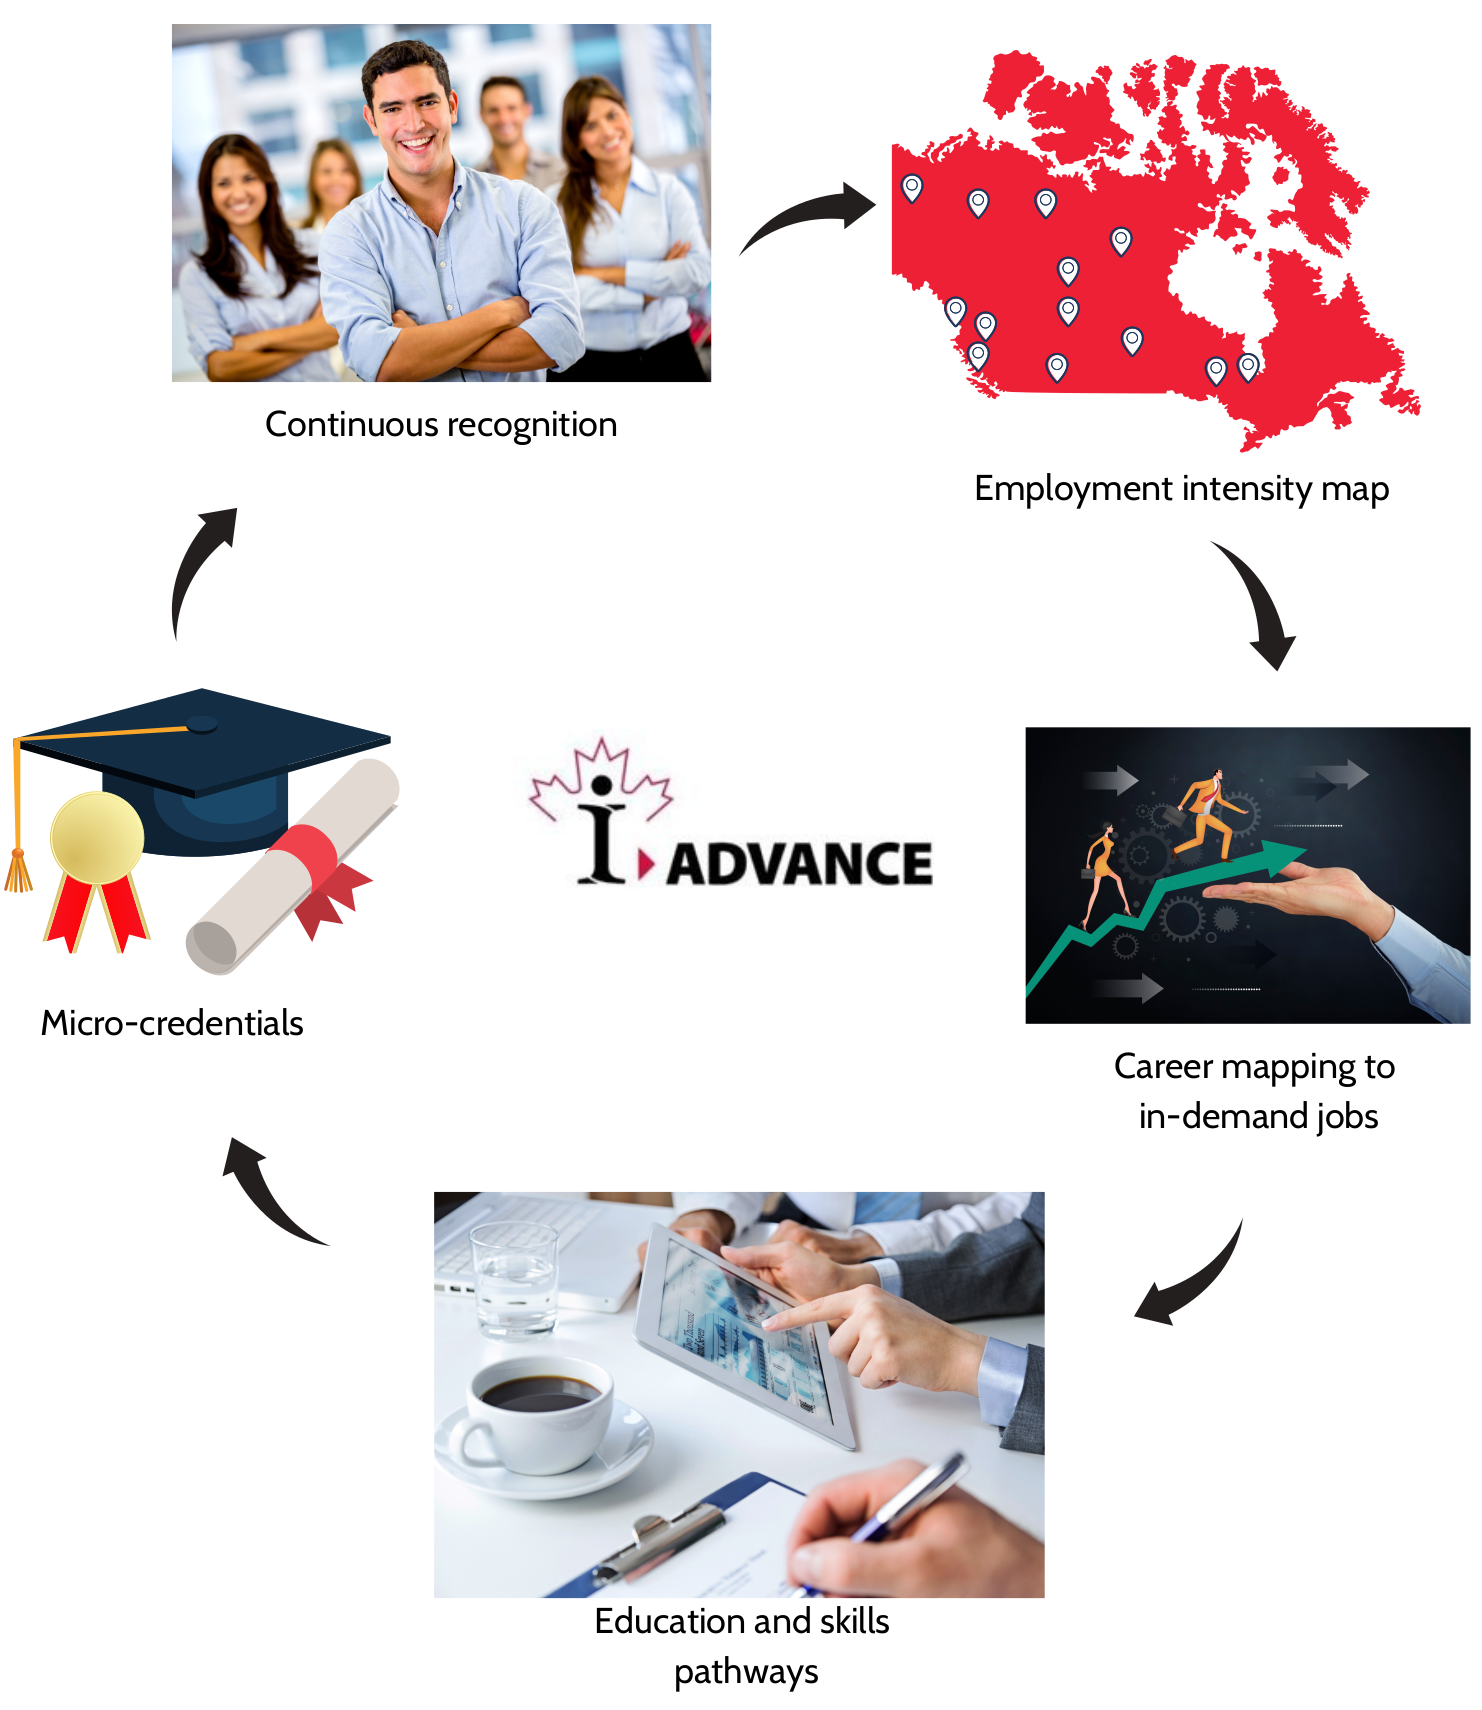
\includegraphics[height=6cm]{../../pics/ictc/iadvance/ictc-iadvance-bigpic}
    \caption{\tiny See the \href{https://www.ictc-ctic.ca/wp-content/uploads/2019/04/iAdvance-ENG-4.1.19.pdf}{iAdvance annoucement}}
	\end{figure}
  \column{0.5\textwidth}
    \vspace{2em}
    The future of Work:
    \begin{itemize}
      \item Dynamic labour market intensity map
      \item Wayfinding
      \item Guided learning path
      \item Self-Sovereign Identity and micro-credential signaling employability
    \end{itemize}
  \end{columns}
}

\frame{
  \frametitle{Call to Action}
  \framesubtitle{from the Think Tank and Innovation Catalyst}
  {\centering\Huge
  Let's partner to accelerate innovation in Canada!\\
  }
  \vspace{2em}
  \normalsize 
  Towards a comprehensive approach to grow the digital economy
  \begin{itemize}
  \item talent development
  \item regulations
  \item new infrastructure (e.g. identity, currency, finance)
  \item new ventures
  \item adoption of technology and new business models
  \end{itemize}
}

% ======================================================================================================
%                                     References
% ======================================================================================================
\section{References}
\frame[allowframebreaks]{
	\frametitle{References}
%	\framesubtitle{Liens utiles}
%	% keyword refers to bib file: references-KEYWORD.bib, and to the Tex file: section-KEYWORD.tex
%	\printbibliography[keyword=inpe]
  \printbibliography
}

\end{document}

